\documentclass{article}
\usepackage{graphicx}

\title{Tugas Pemrograman 2}
\begin{figure}
    \begin{center}
        
\includegraphics[width=6cm]{poltekpos.jpg}
    \end{center}
\end{figure}
\author{Annisa Khairani Febrianti}
\date{1184071}

\begin{document}

\maketitle

\section{Sejarah Python}
\hspace{1cm}{Python diciptakan oleh Guidovan Rossum yang pertama kali di Centrum wiskunde dan Informatica (CWI), Pada awal tahun 1990-an di negara Belanda. Bahasa python terisnpirasi dari salah satu bahasa pemrograman yaitu ABC dan bersifat Open Source.Pada tahun 1995 Guido membuat bahasa Python di Corporation for national research initiative(CNRI)di negara Virginia Amerika, sedangkan pada bulan Mei tahun 2000 Guido dan para timnya pindah ke Beopen.com dan membentuk sebuah tim baru yang bernama Be Open Python Labs. Pada Tahun 2001 dibentuklah sebuah organisasi yaitu "Python Software Foundation"(PSF) yang artinya Organisasi "Nirlaba". Python ini adalah salah satu dari bahasa pemrograman skrip.}

\section{Perbedaan Python 2 dan 3}
\hspace{1cm}{Adapun perbedaan dari python 2 dan python 3 tidaklah jauh berbeda dengan python yang lainnya.Namun, ada beberapa yang sedikit berbeda. Yuk, kita lihat perbedaannya di bawah ini.}
\subsection{Python 2}
\hspace{1cm}{Python 2 dibikin pada akhir tahun 2000, Python ini dinilai lebih transparan dan inklusif dari pengembangan software python lainnya. python ini di dukung dengan adanya PEP- Python Enchonment proposal. Python ini dilengkapi dengan fitur Programatikal, salah satunya adalah cycle-detecting, garbage collector yang berfungsi untuk mengotomasi manajemen memori. Unifikasi pada tipe data python dan class dari satu hirarki ini terjadi pada rilis python 2.2.}
\newpage
\subsection{Python 3}
\hspace{1cm}{Python 3 dibikin pada akhir tahun 2008 dan fokus untuk melakukan perapian pada sebuah codebase dan menghapuskan sebuah duplikasi atau redudancy.Python 3 merupakan pengembangan dari python 2 dan perubahan tersebarnya adalah untuk memasukkan salah satu statemen print ke dalam built-in function. hal ini para pengguna python lebih banyak menggunakan versi 2 daripada versi 3 karena didalamnya lebih banyak library yang tersedia, tetapi setelah semua tim mengembangkan versi 3 dan menjelaskan terhadap versi 2 yang akan segere di berhentikan, dan menyuruhkan para pengguna python menggunakan versi 3 dan penerapannya semakin menigkat.}

\section{Implementasi dan Penggunaan Python di Perusahaan Dunia}
\hspace{1 cm}{Adapun 5 perusahaan yang menggunakan bahasa python didunia yang berfungsi untuk memecahkan suatu masalah yang rumit dan membuat suatu aplikasi yang top dan terkenal, salah satu 5 perusahaan tersebut yaitu: }
\item 1.{Sportify, sportify tersebut menyediakan pelayanan musik streaming yang memanfaatkan sebuah analisis data dan terkenal pada Backend sportify terdapat service yang berkomunikasi melewati 0MQ (Z00 MQ) yang artinya Framework dan library Open Source yang digunakan untuk mengkonsolidasi eror secara cepat.}
\item 2. {Google, Diawal pembuatan google sudah menggunakan bahasa python tersebut, salah satu bahasa python nya adalah "Python where we can, C++ where we must".}
\item 3. {Industrial Light and Magic, ILM dibuat pada tahun 1975 yang artinya studio special efek ilon yang dibuat dengan bahasa pemrograman C dan C++.}
\item 4. {Netflix, Adalah sebuah aplikasi yang Central Alert Gateway dan menelusuri riwayat perubahan pengaturan pada sebuah keamanan.}
\item 5. {Instagram}

\newpage
\section{INSTALASI}
\subsection{Instalasi Python 3}
\begin{enumerate}
    \item Pertama-tama kita download Anaconda terlebih dahulu sesuai dengan OS yang anda pakai, anda dapat mengunduhnya di https://www.python.org/downloads/release/python-370.
    \item Setelah terunduh, klik dua kali pada file instalasi tersebut. Lalu akan muncul tampilan seperti ini, klik next.
        \begin{figure}[h]
            \centerline{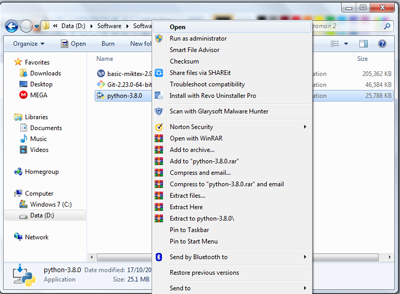
\includegraphics[width=8cm]{image/1.png}}
        \end{figure}
    \item kemudian kita Klik I agree, untuk menyetujui license instalasi Anaconda.
        \begin{figure}[h]
            \centerline{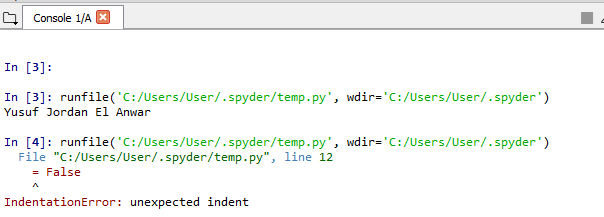
\includegraphics[width=8cm]{image/2.png}}
        \end{figure}
    \newpage \item Lalu pilih installation tipe,  terus kita klik just me (yang akan kita rekomendasikan).
        \paragraph{}
            \centerline{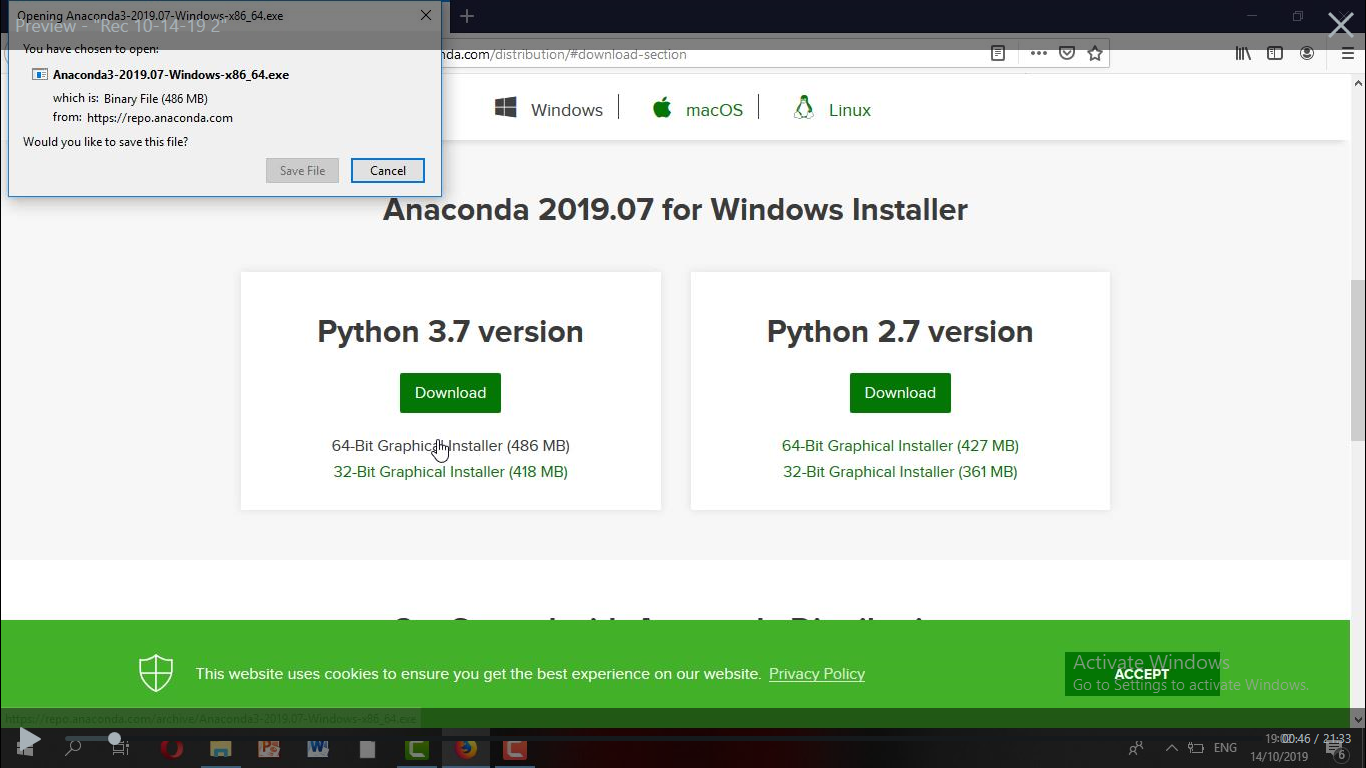
\includegraphics[width=8cm]{image/3.png}}
    \item Lalu pilih tempat atau lokasi direktori untuk instalasi Anaconda, lalu kita klik next.
        \begin{figure}[h]
            \centerline{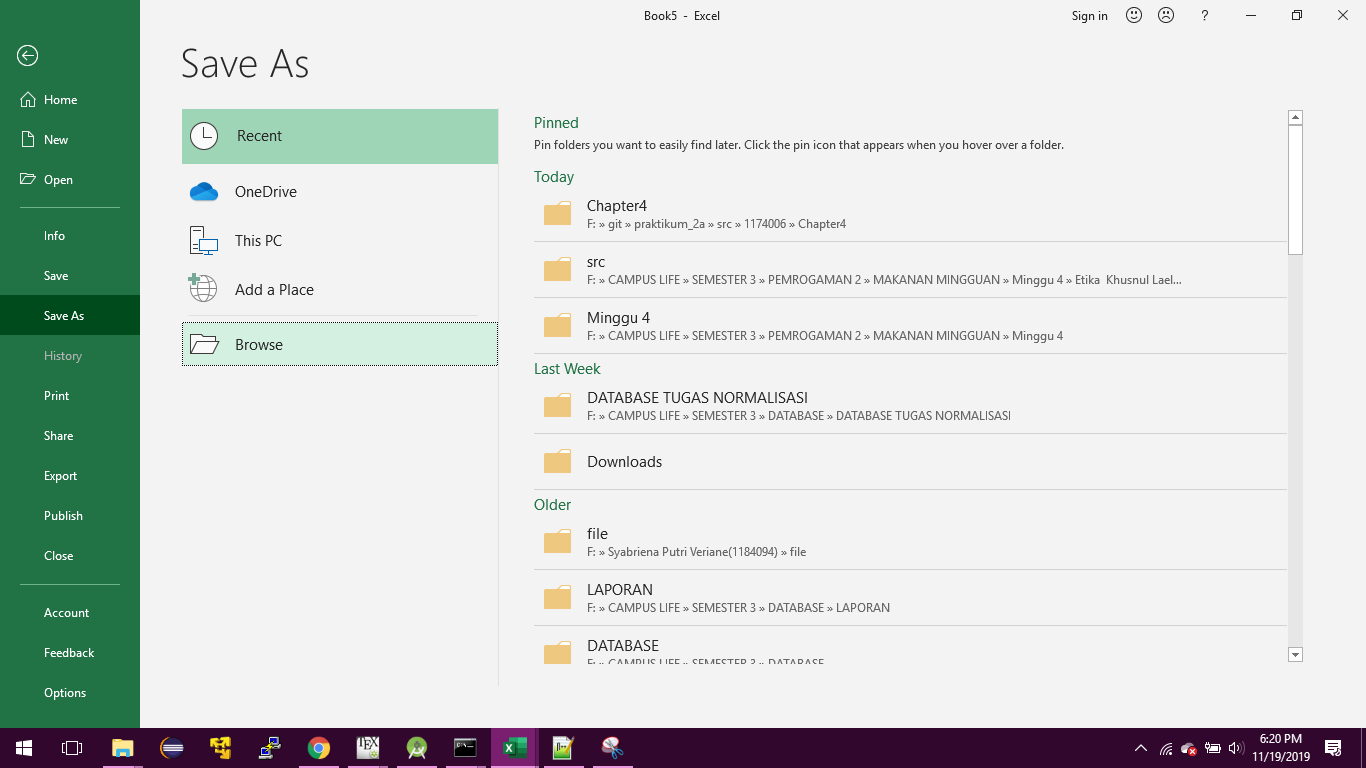
\includegraphics[width=8cm]{image/4.png}}
        \end{figure}
    \item Untuk advance option, kita pilih dua opsi tersebut. Tunggu hingga instalasi Anaconda selesai.
        \begin{figure}[h]
            \centerline{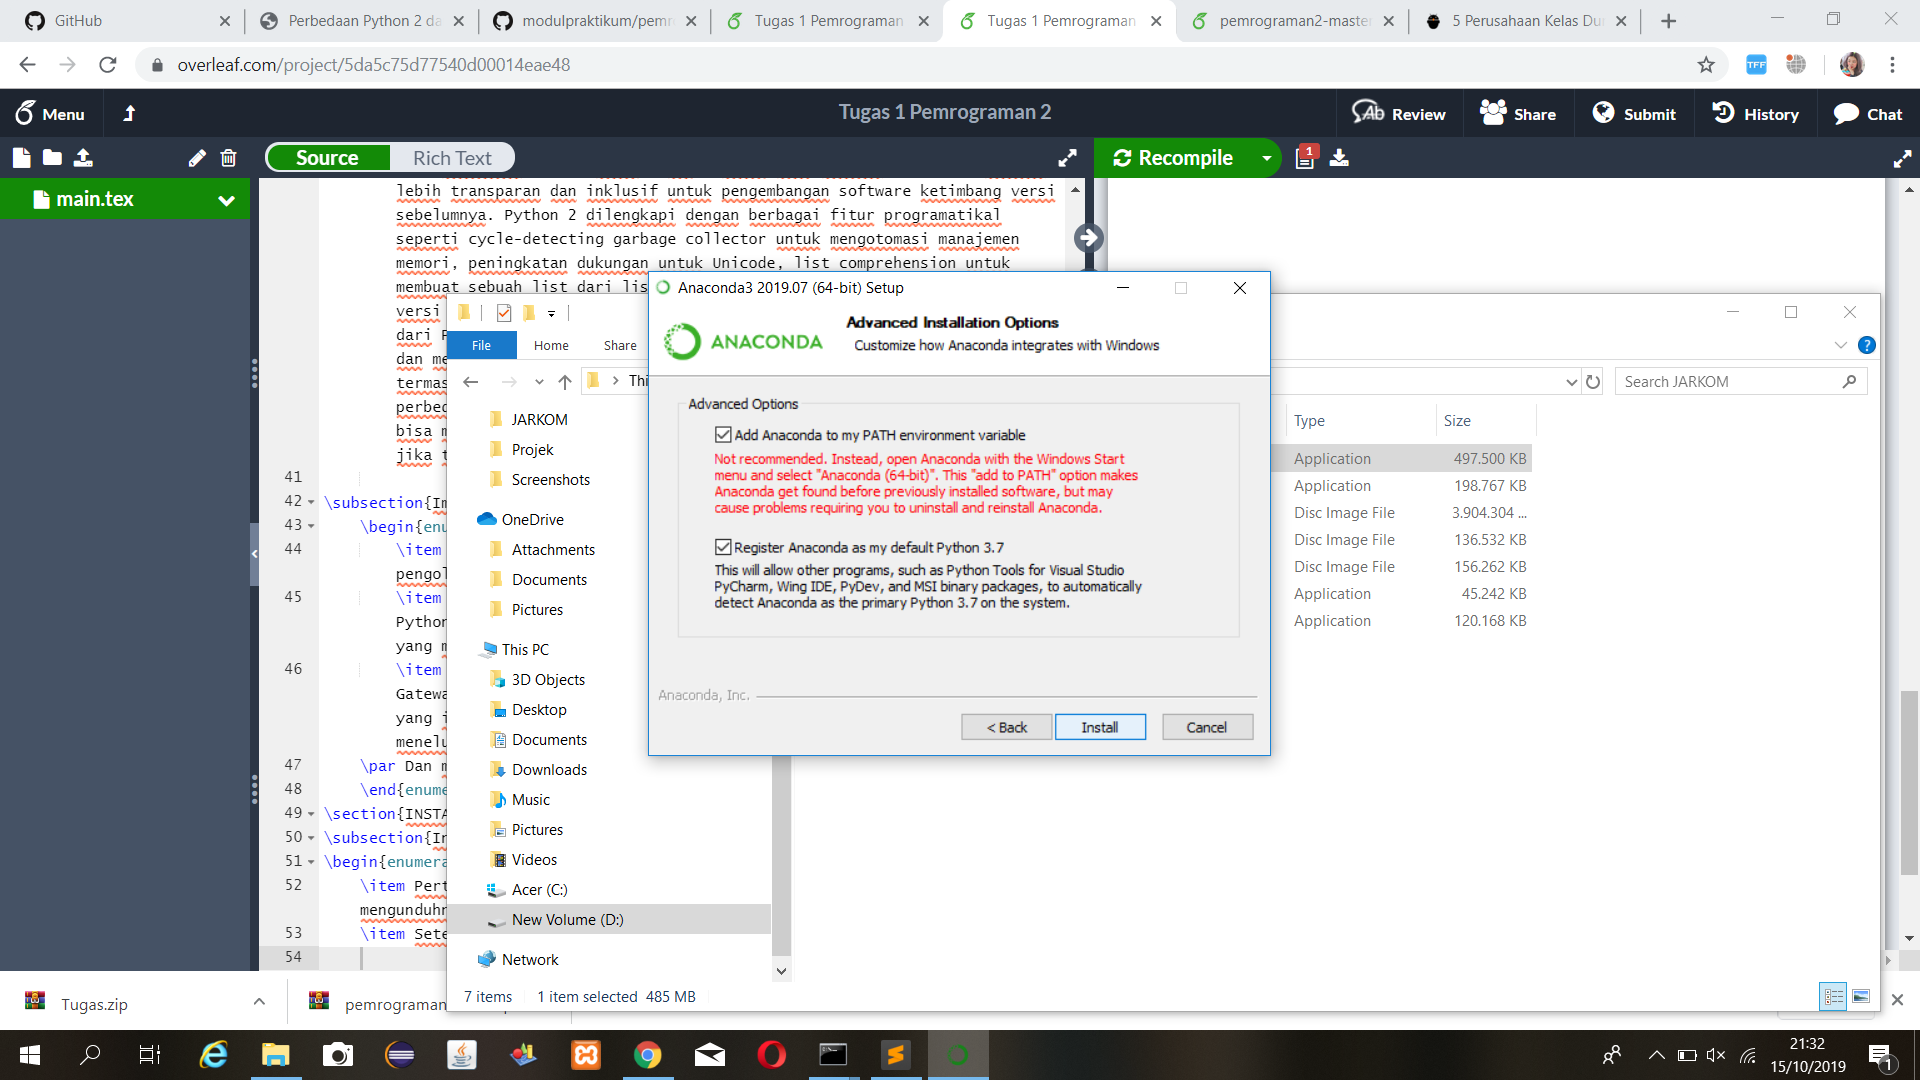
\includegraphics[width=8cm]{image/5.png}}
        \end{figure}
\end{enumerate}

\newpage
\subsection{Instalasi PIP}
\begin{enumerate}
    \item Pertama-tama kita buka Anaconda promt atau dengan meng-klik tombol jendela windows dan huruf R secara bersamaan, maka akan menampilkan gambar seperti di bawah ini. Pilih cmd kemudian kita tekan OK.
        \begin{figure}[h]
            \centerline{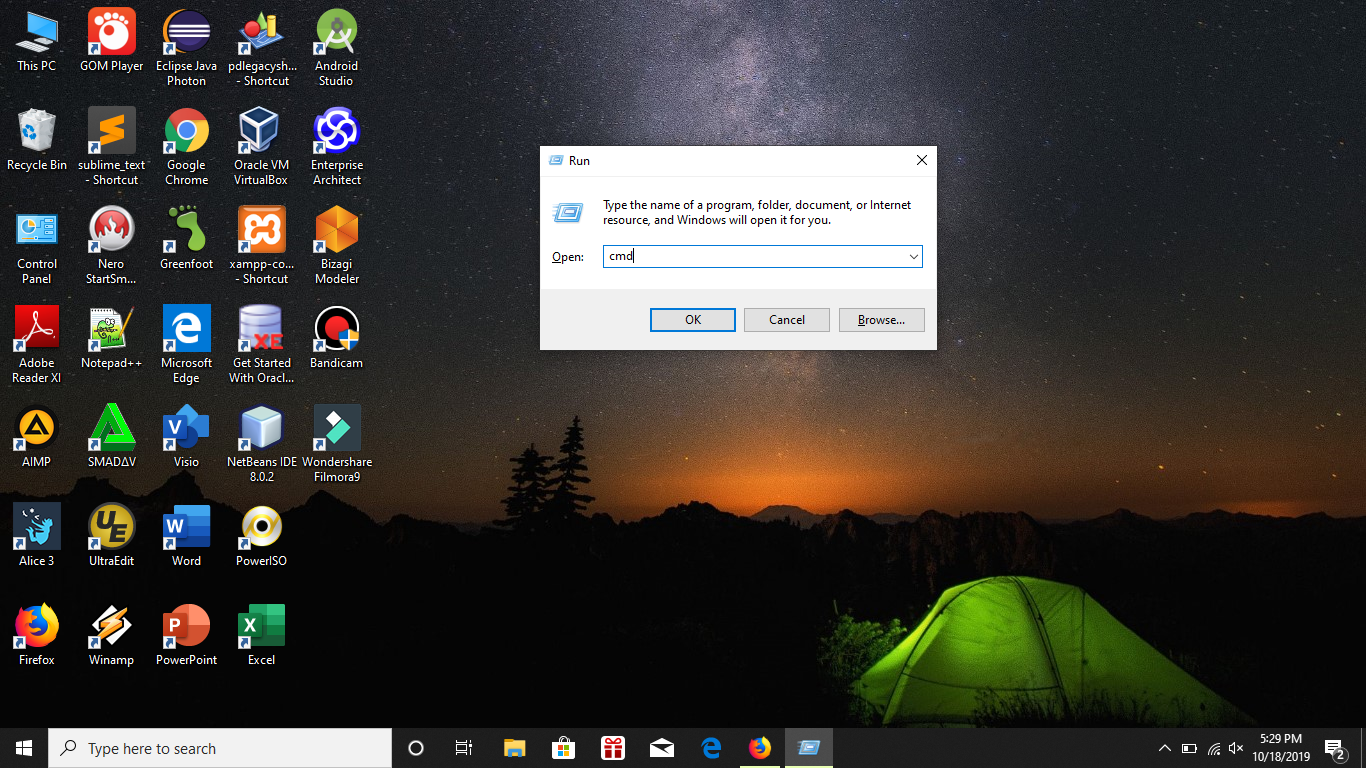
\includegraphics[width=8cm]{image/cmd.png}}
        \end{figure}
    \item Lalu kita ketikkan pip install requests.
        \begin{figure}[h]
            \centerline{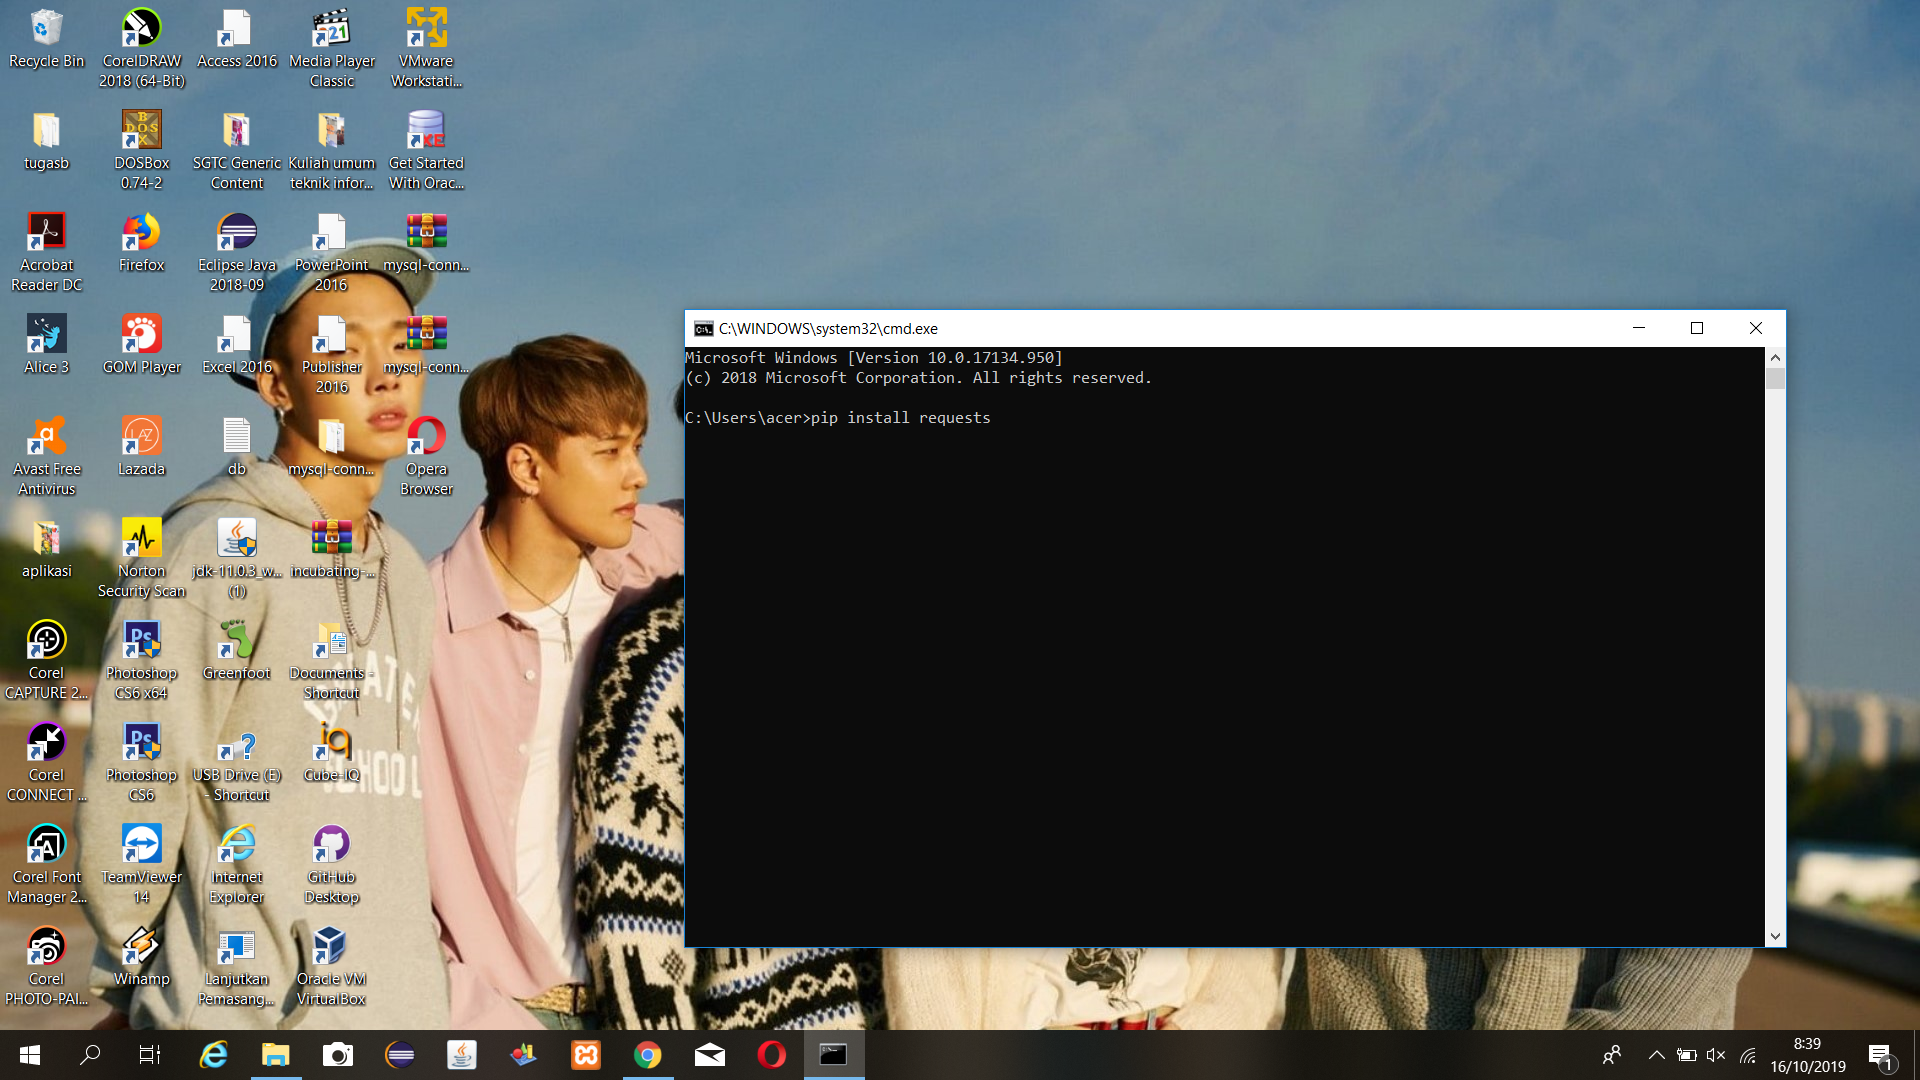
\includegraphics[width=8cm]{image/pip.png}}
        \end{figure}
    \newpage \item Jika berhasil maka akan keluar seperti berikut ini, jika gagal maka akan muncul error.
            \paragraph{}
            \centerline{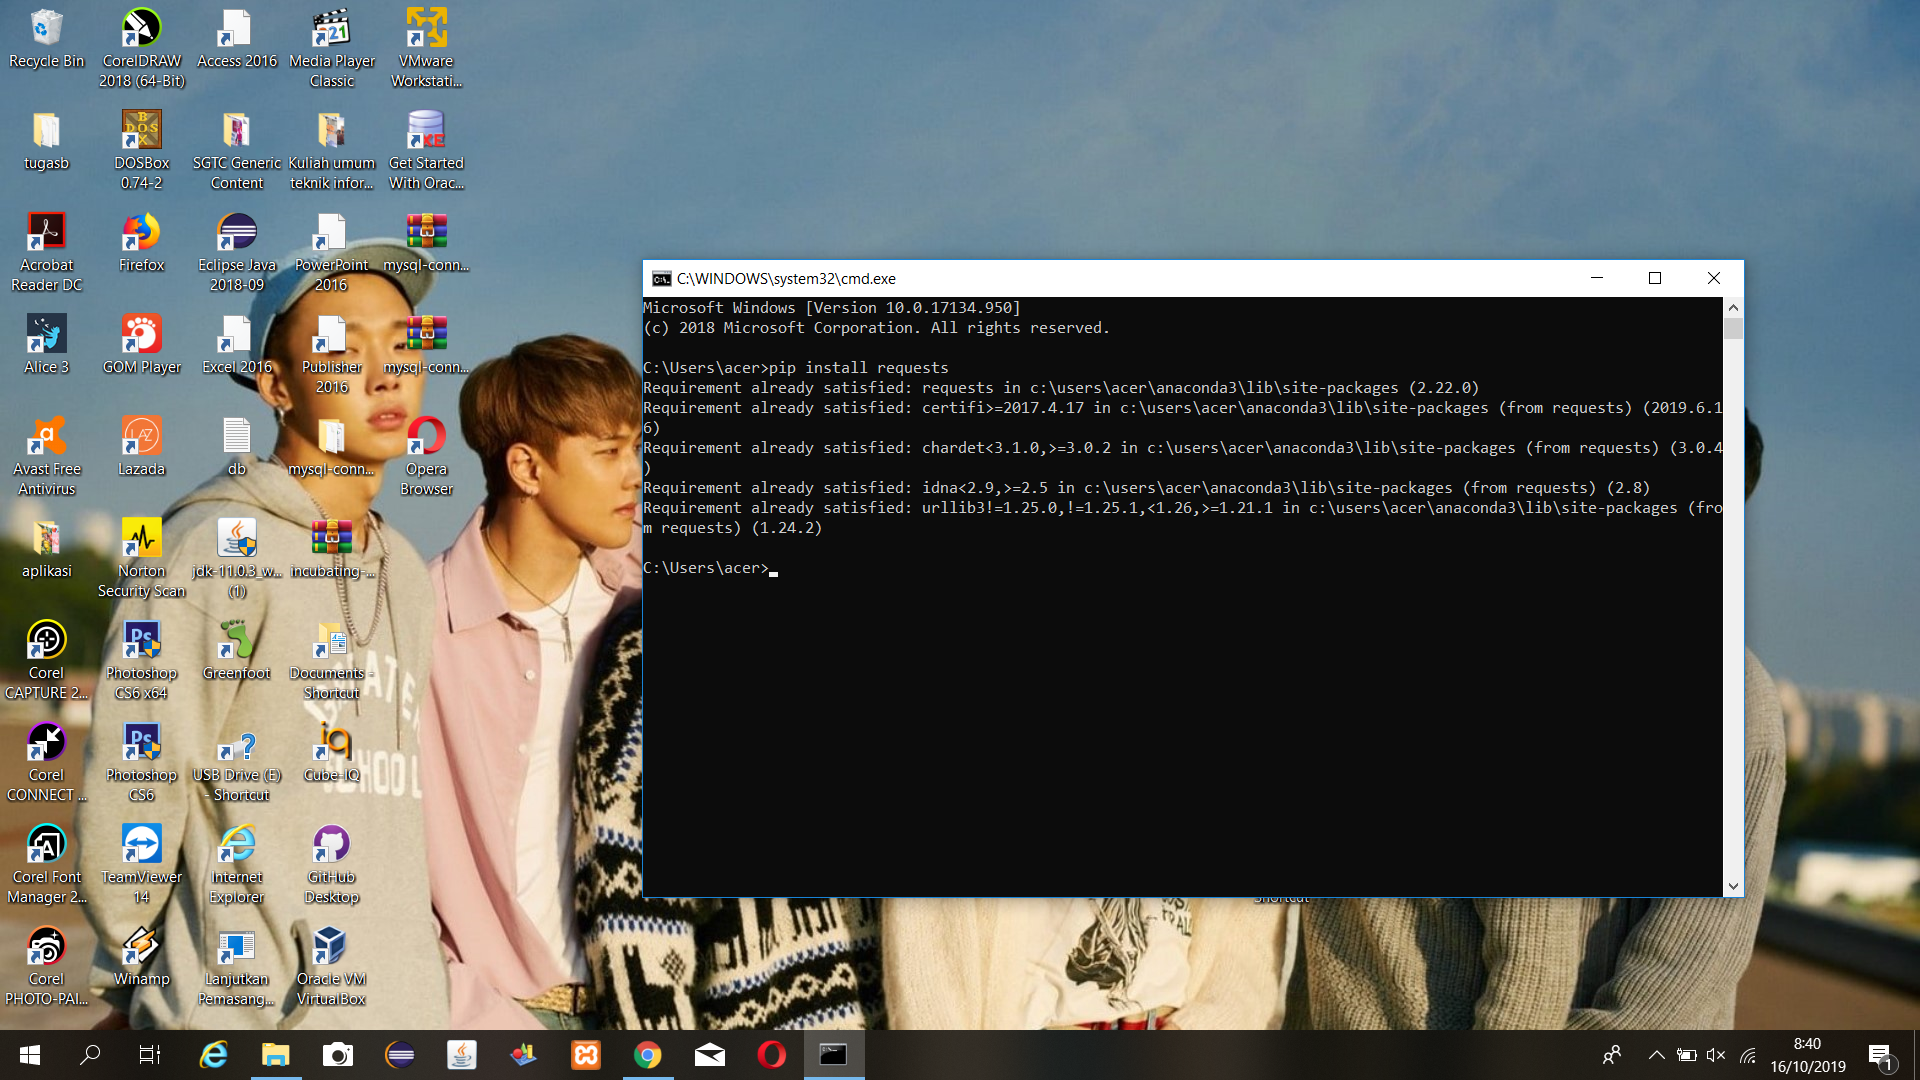
\includegraphics[width=8cm]{image/pipberhasil.png}}
\end{enumerate}

\subsection{Setting Environment}
\begin{enumerate}
    \item Pertama-tama kita masuk ke control panel lalu pilih system dan security
        \begin{figure}[h]
            \centerline{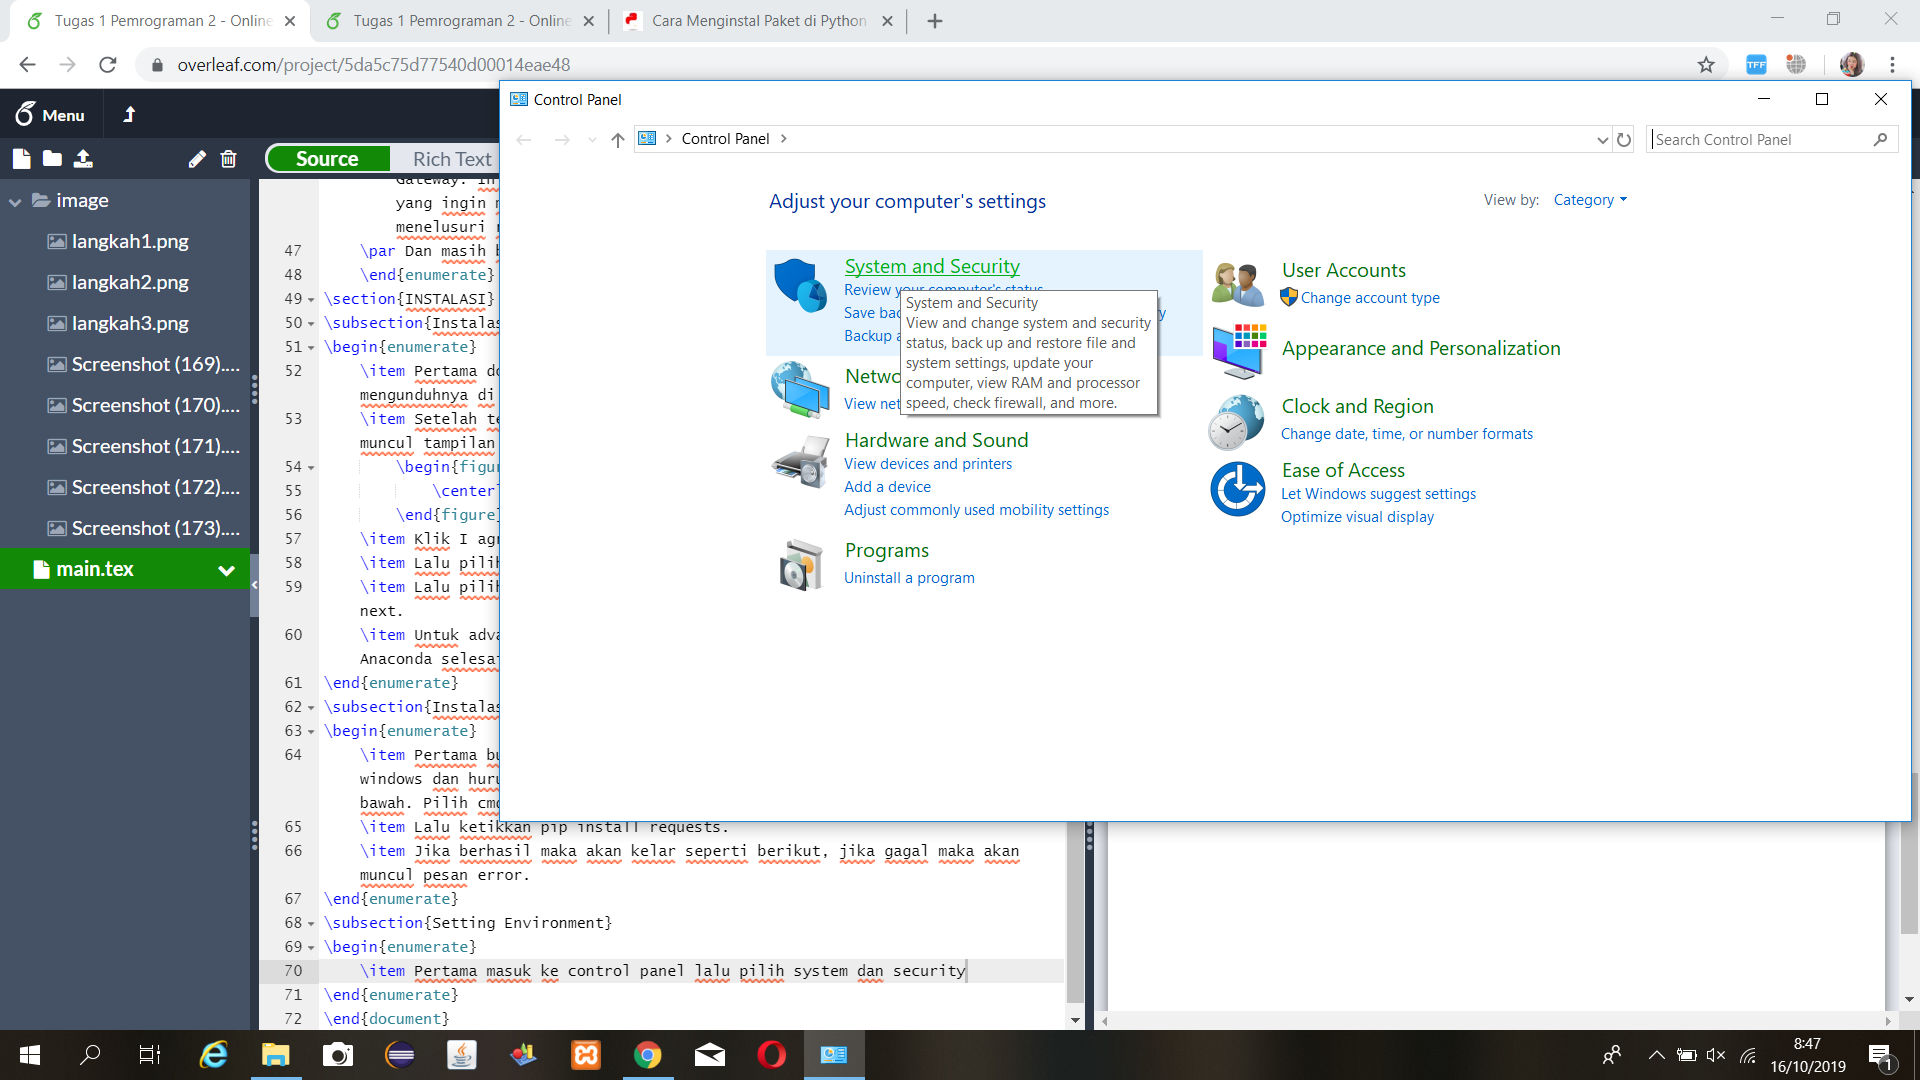
\includegraphics[width=8cm]{image/cpanel.png}}
        \end{figure}
    \item Lalu kita pilih Security and Maintanance
        \begin{figure}[h]
            \centerline{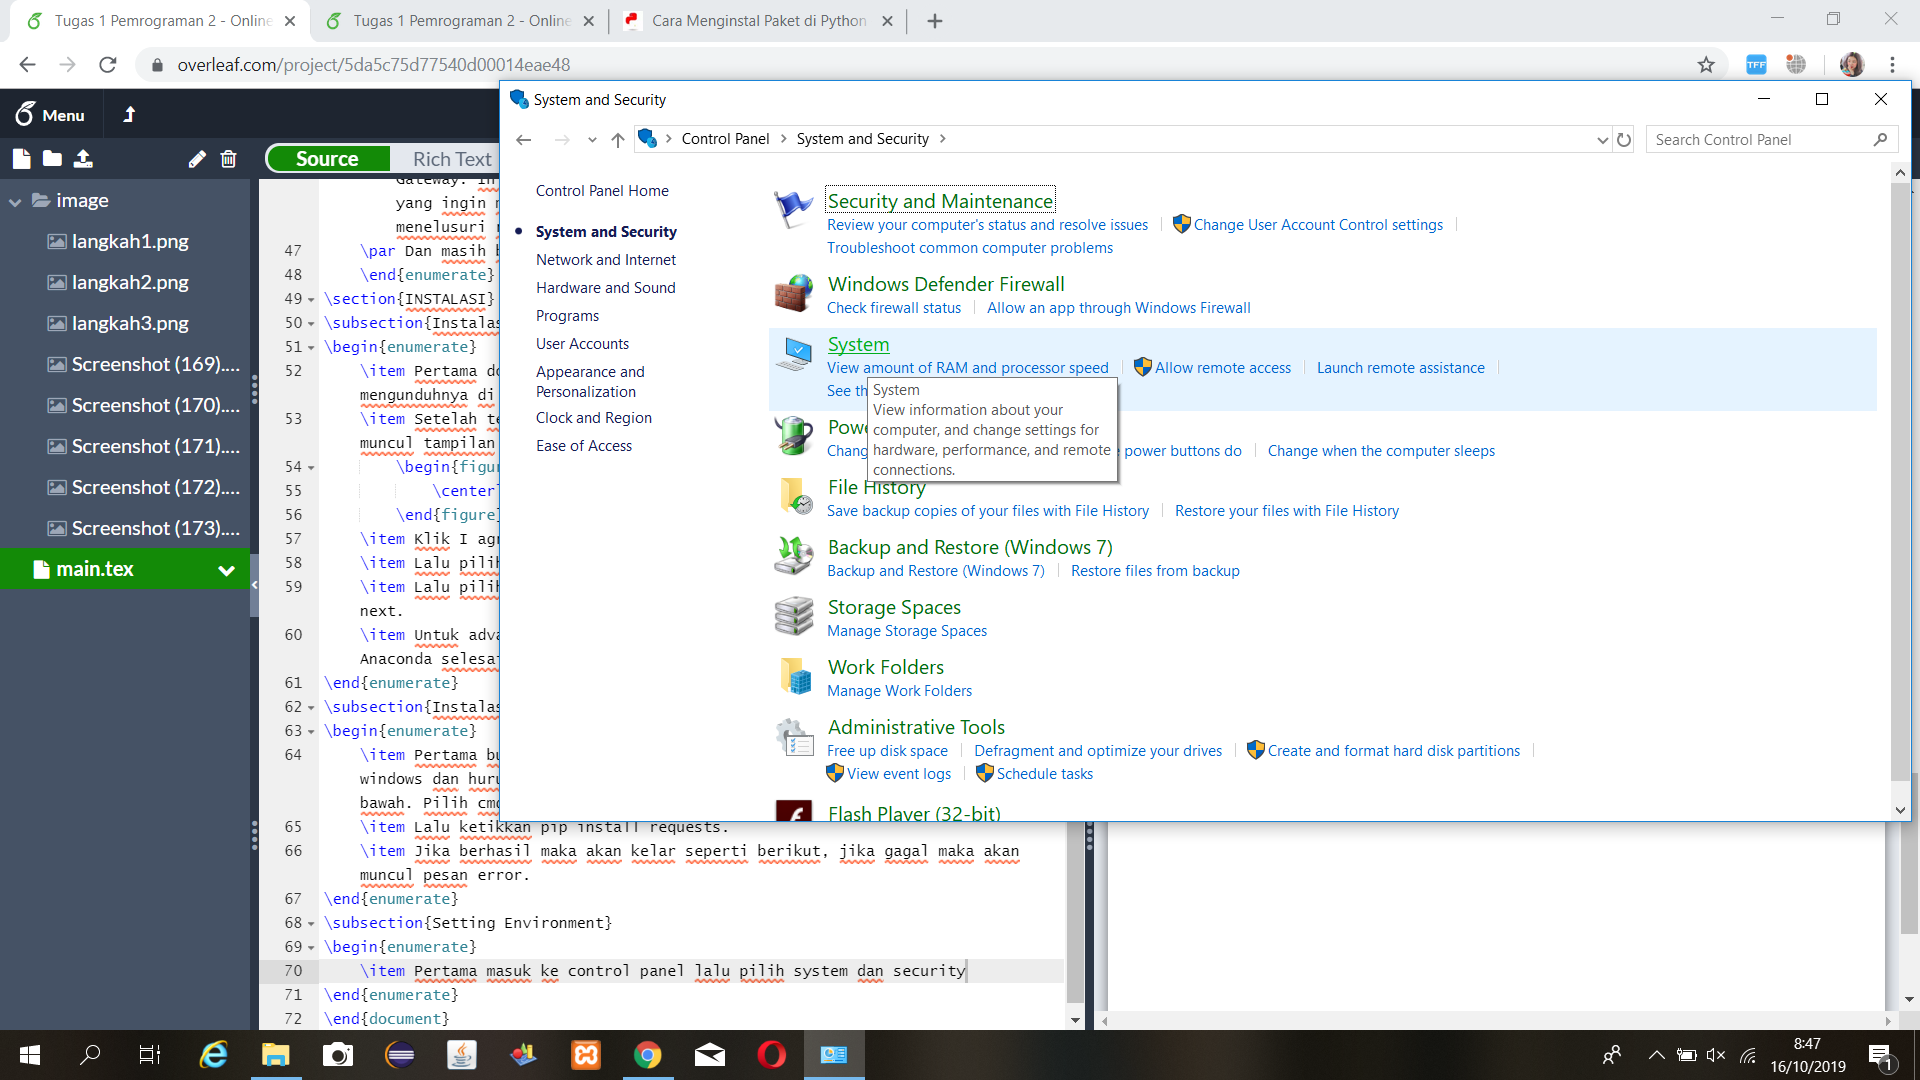
\includegraphics[width=8cm]{image/securityandmain.png}}
        \end{figure}
    \item Setelah itu kita pilih System dan Advanced System Settings.
            \paragraph{}
            \centerline{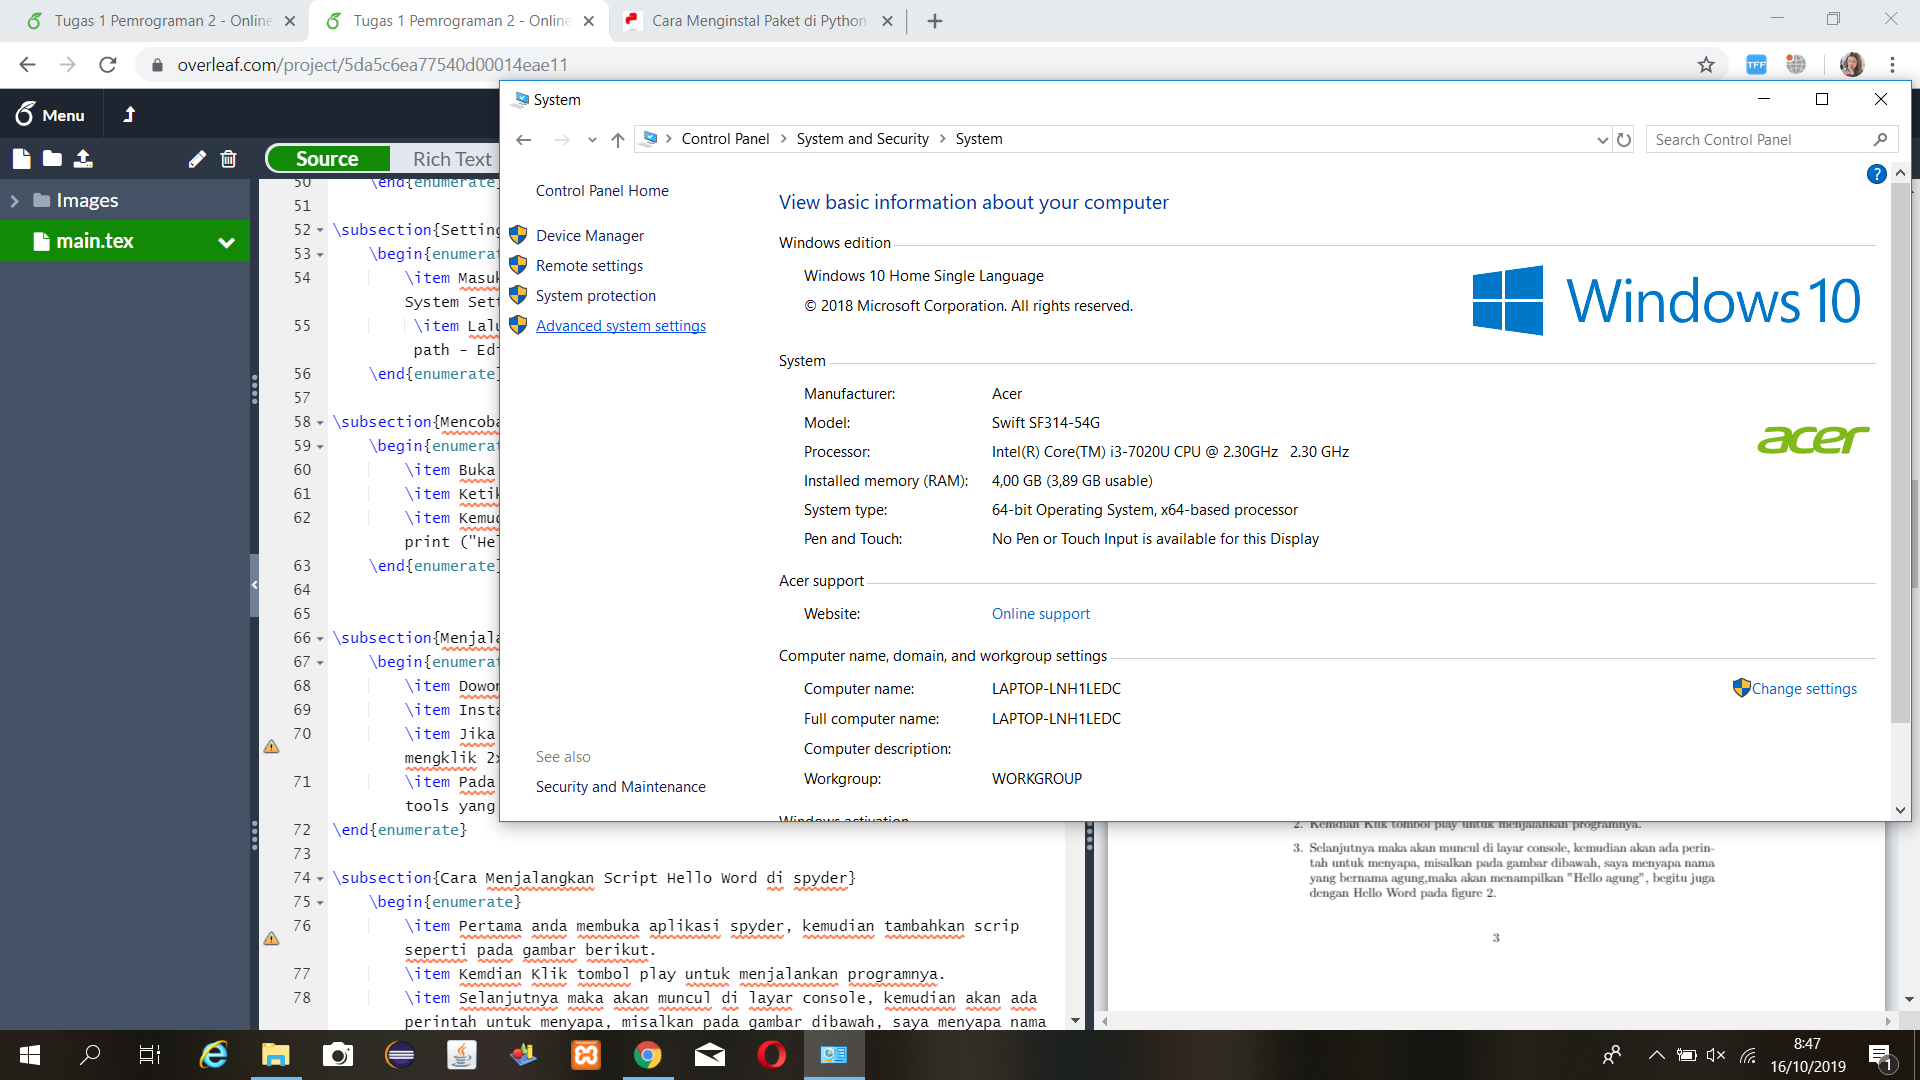
\includegraphics[width=8cm]{image/advanced.png}}
    \newpage \item Lalu kita pilih lagi environment variables, lalu di System Variables kita klik path-Edit-New-C:/Python3/Scripts lalu kita klik OK.
        \begin{figure}[h]
            \centerline{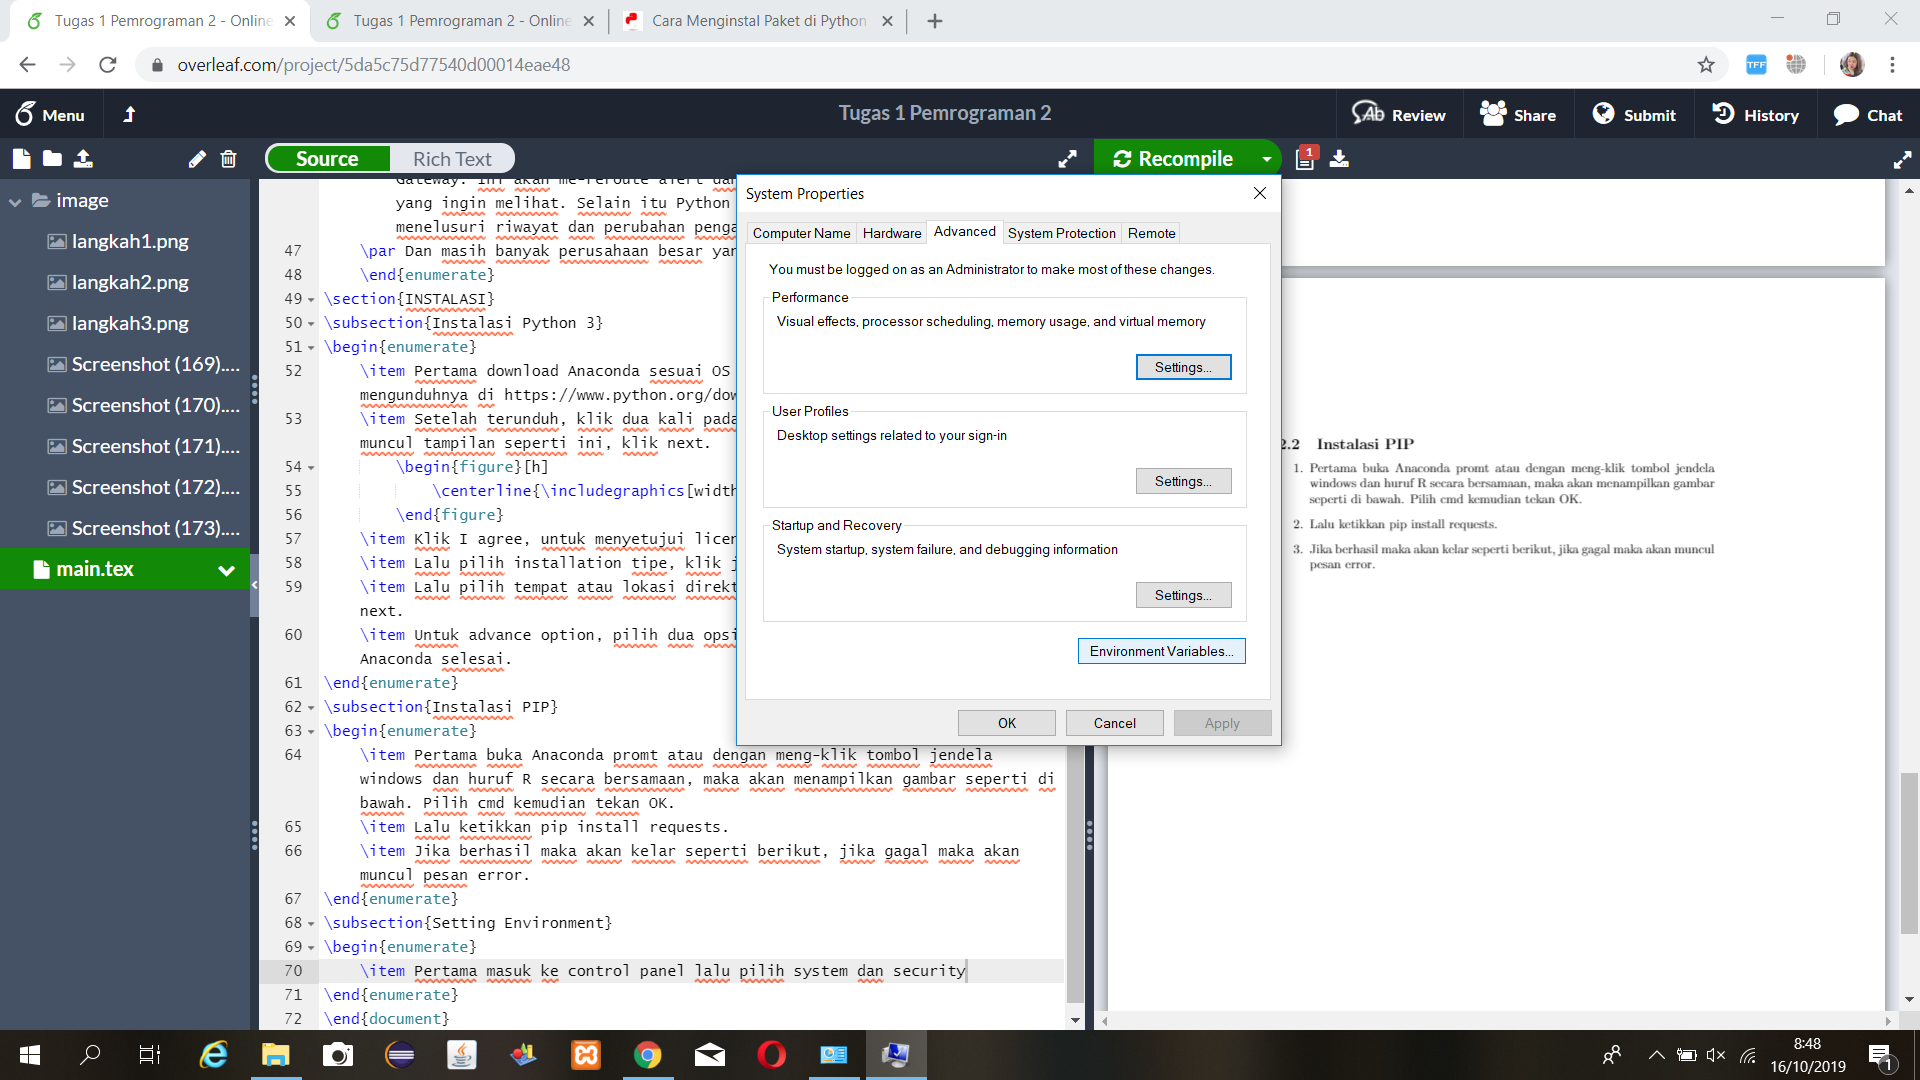
\includegraphics[width=8cm]{image/environtmentvar.png}}
        \end{figure}
        \begin{figure}[h]
            \centerline{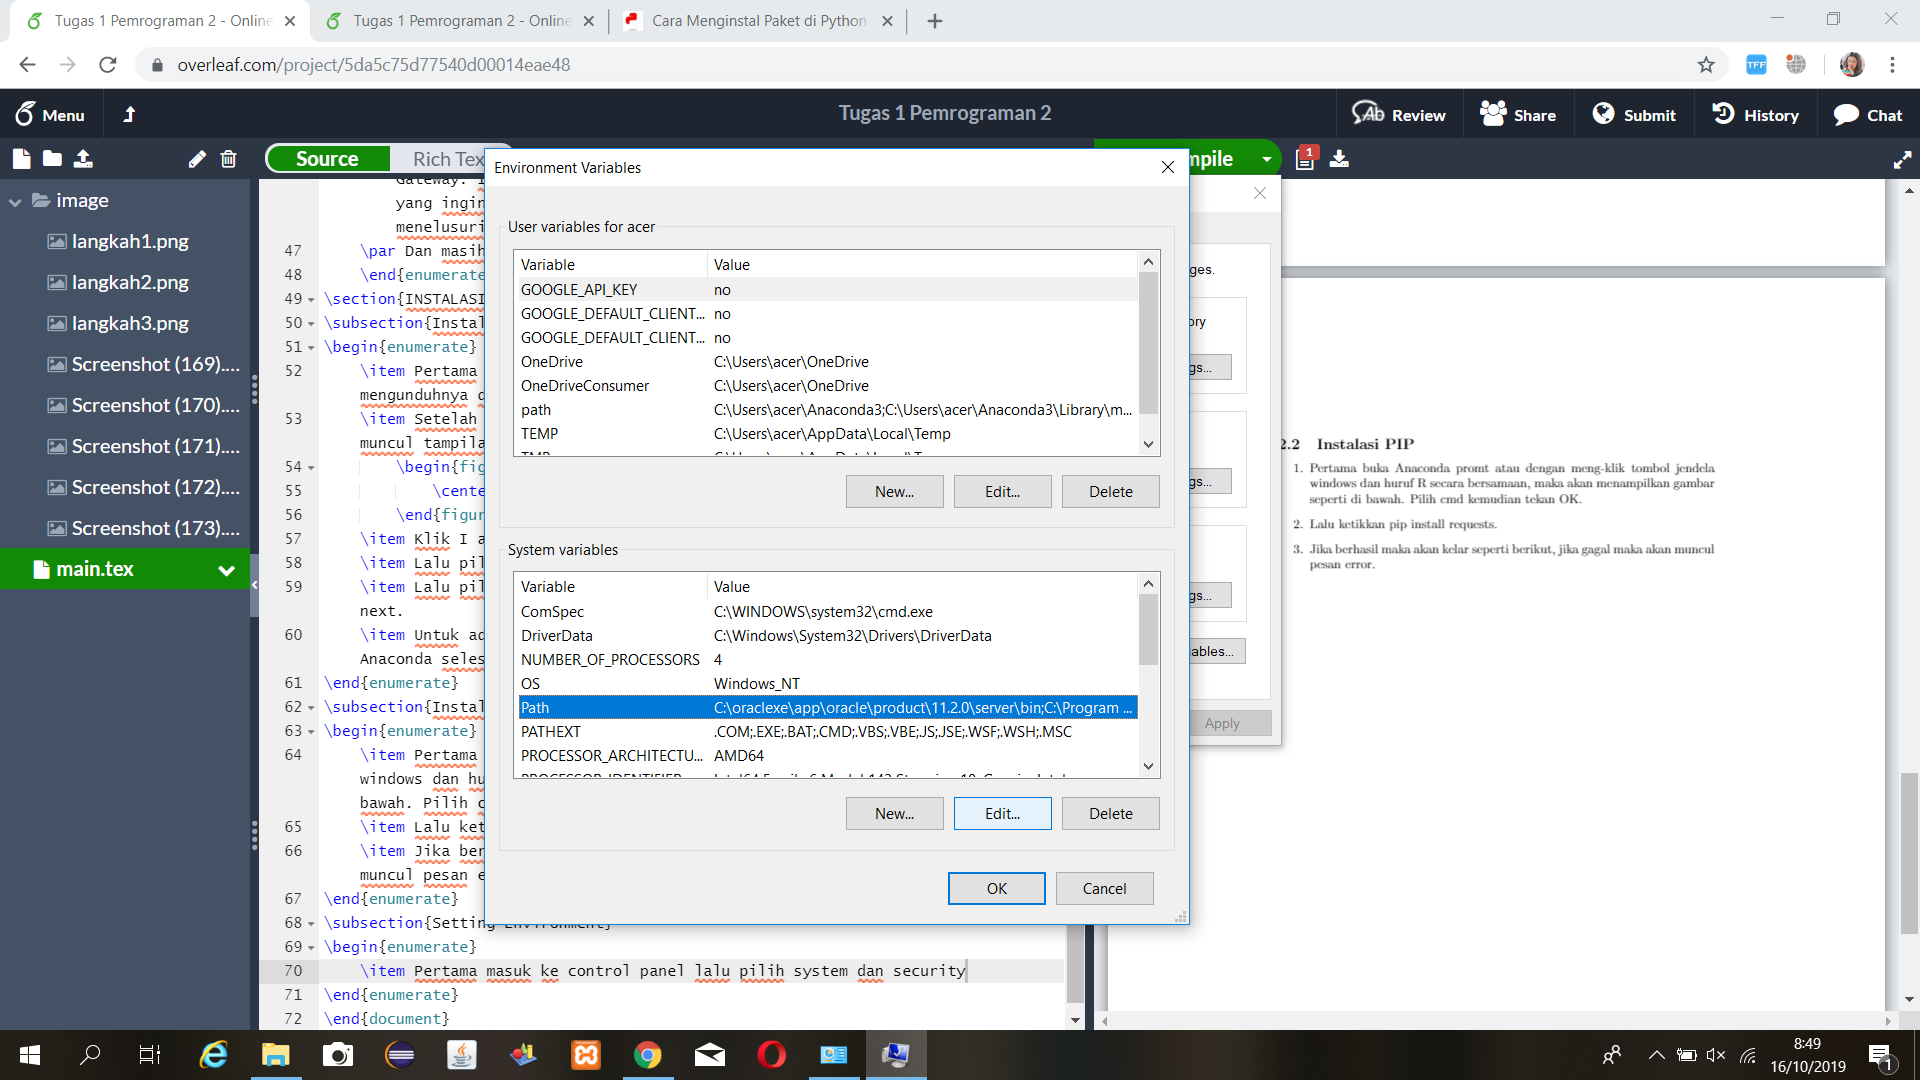
\includegraphics[width=8cm]{image/pathedit.png}}
        \end{figure}
        \paragraph{}
            \centerline{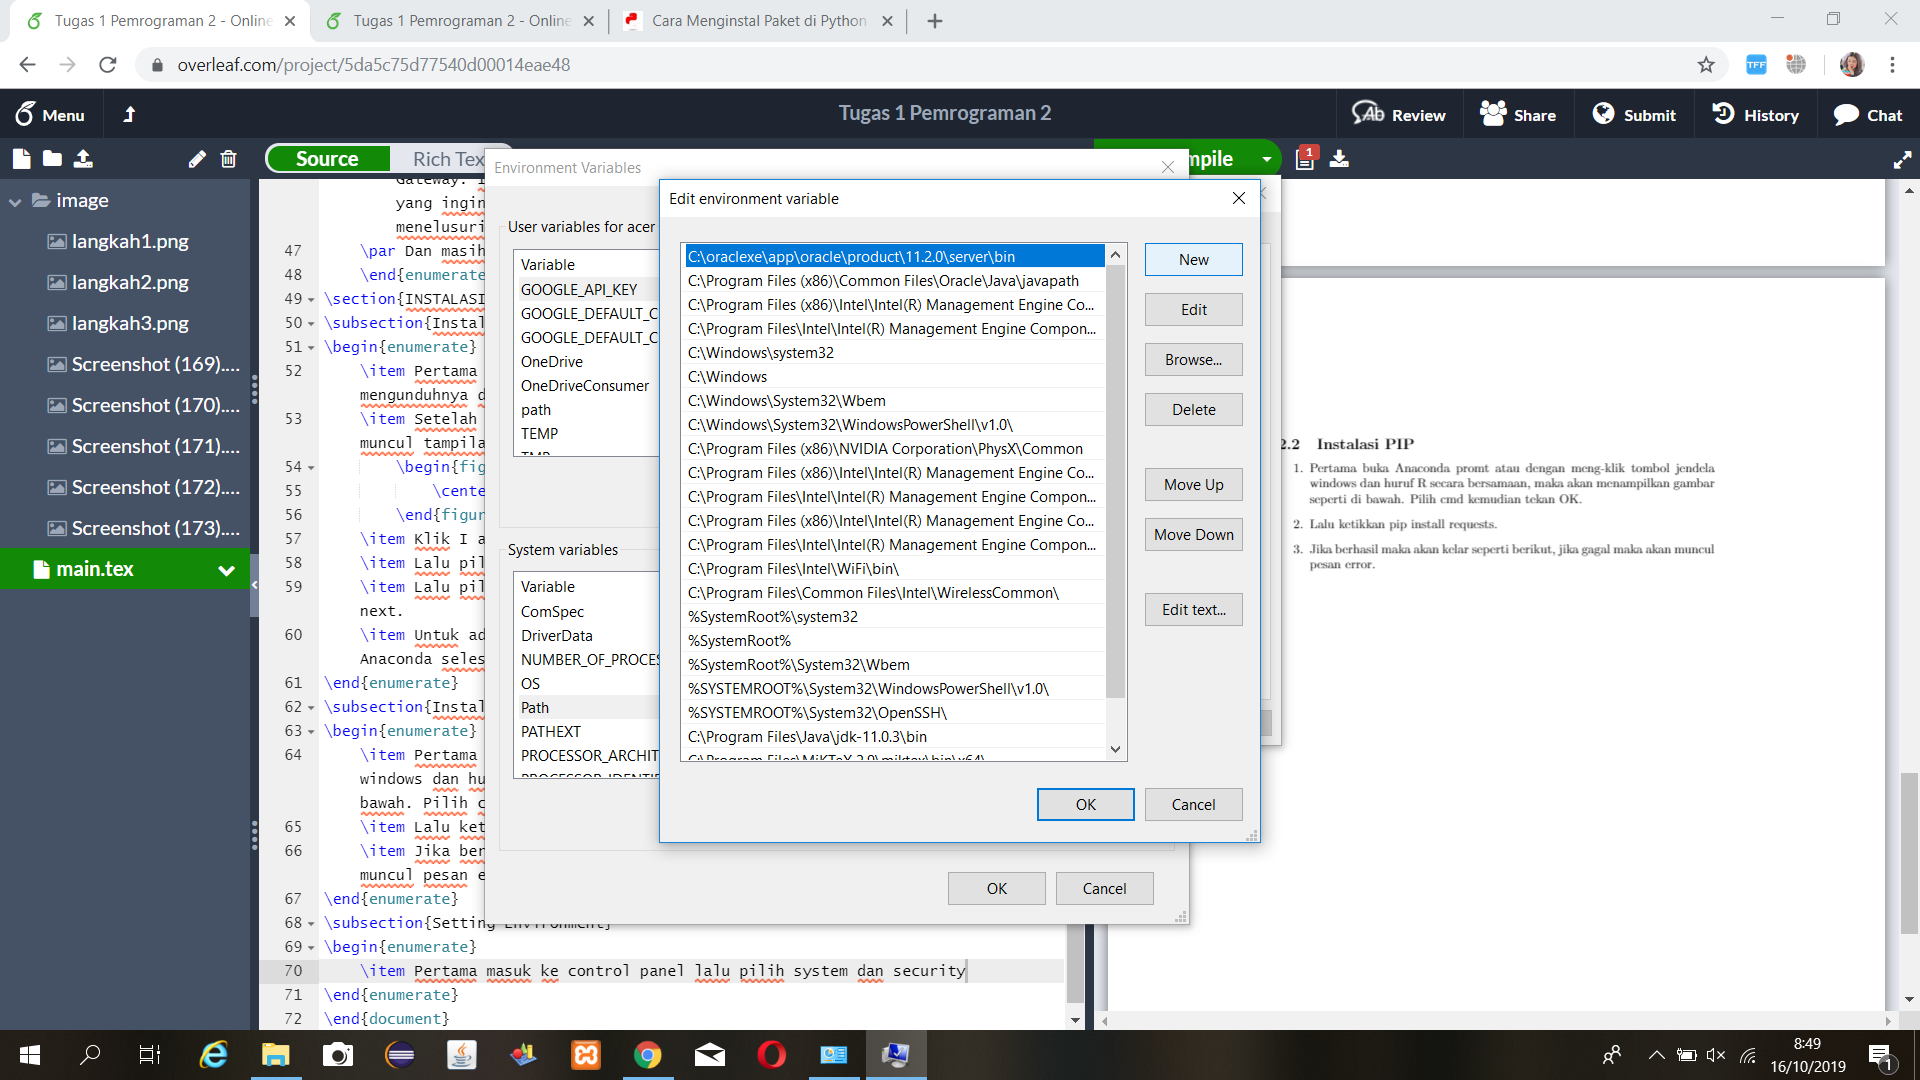
\includegraphics[width=8cm]{image/new.png}}
        \paragraph{}
            \centerline{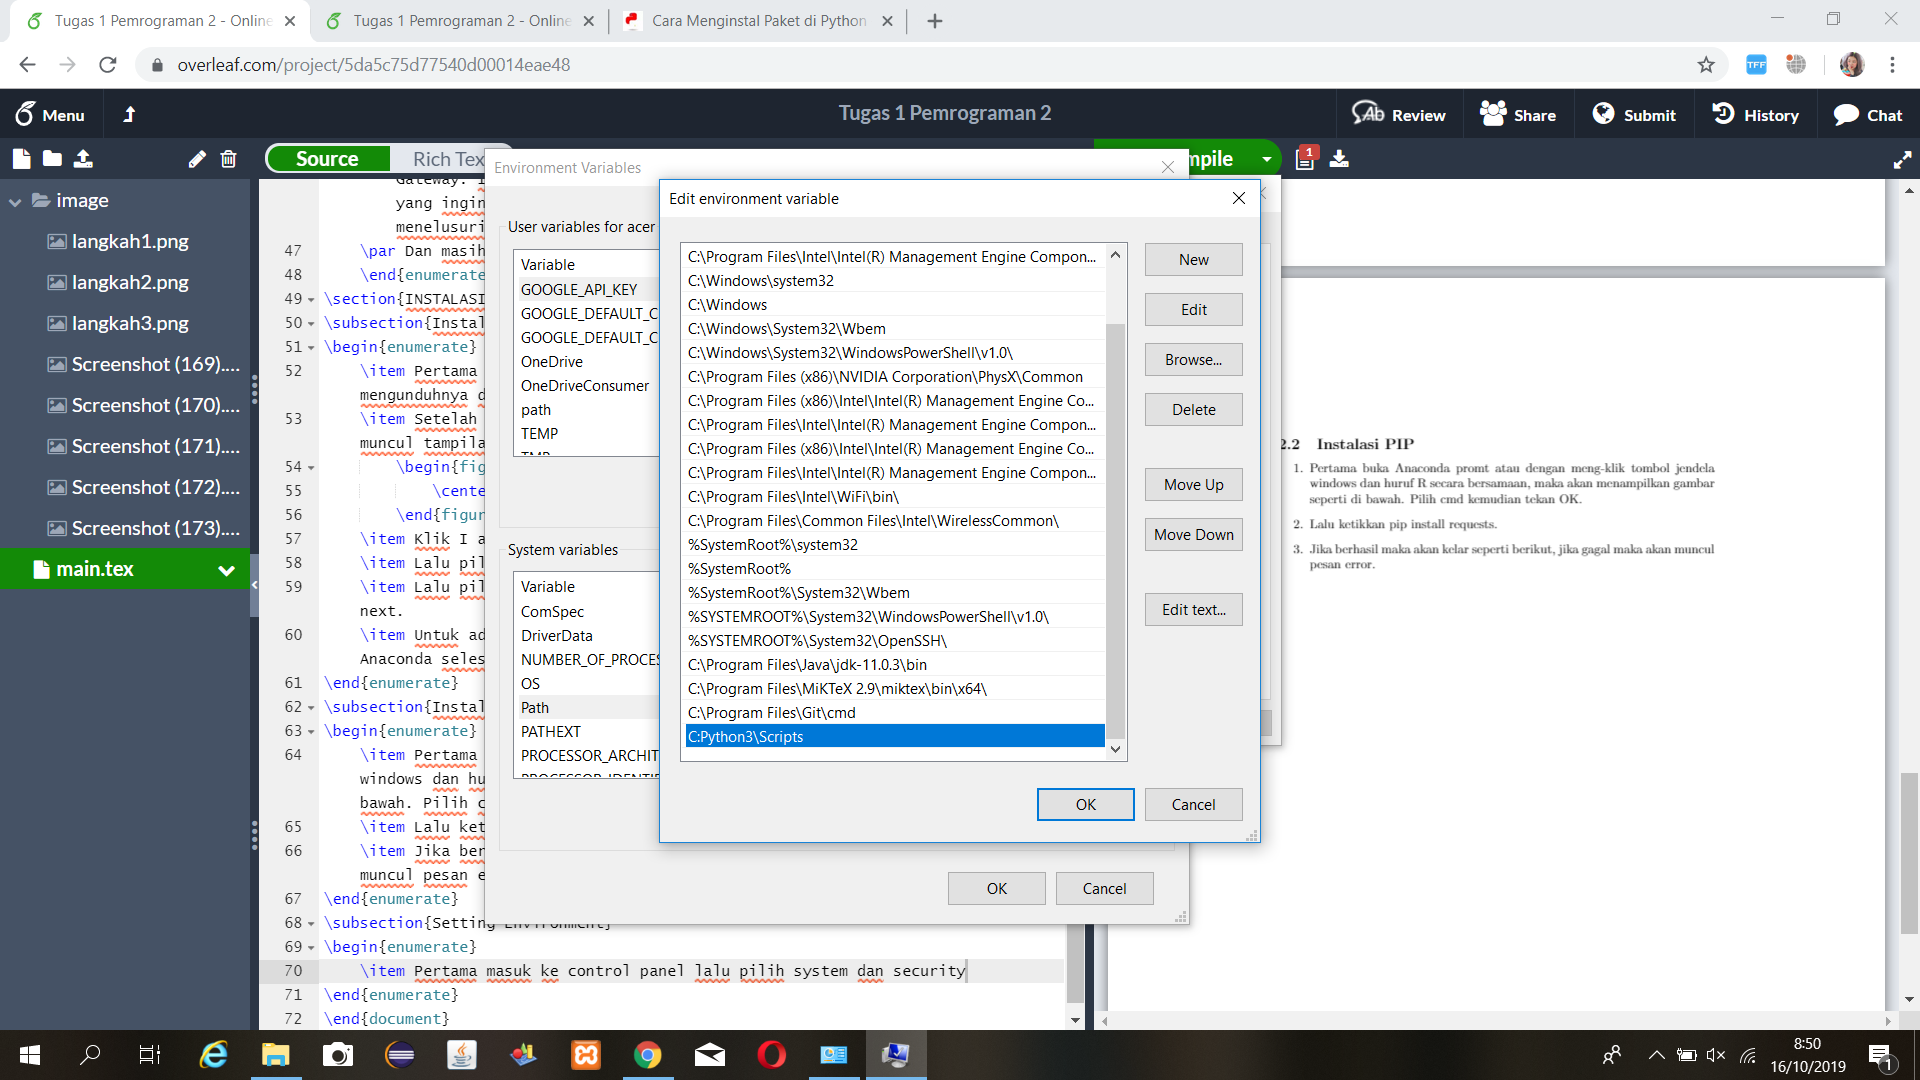
\includegraphics[width=8cm]{image/pathnewok.png}}
\end{enumerate}
\subsection{Mencoba Interpreter/CLI pada CMD}
\begin{enumerate}
    \item Pertama kita buka Cmd terlebih dahulu pada PC/Laptop anda.
        \begin{figure}[h]
            \centerline{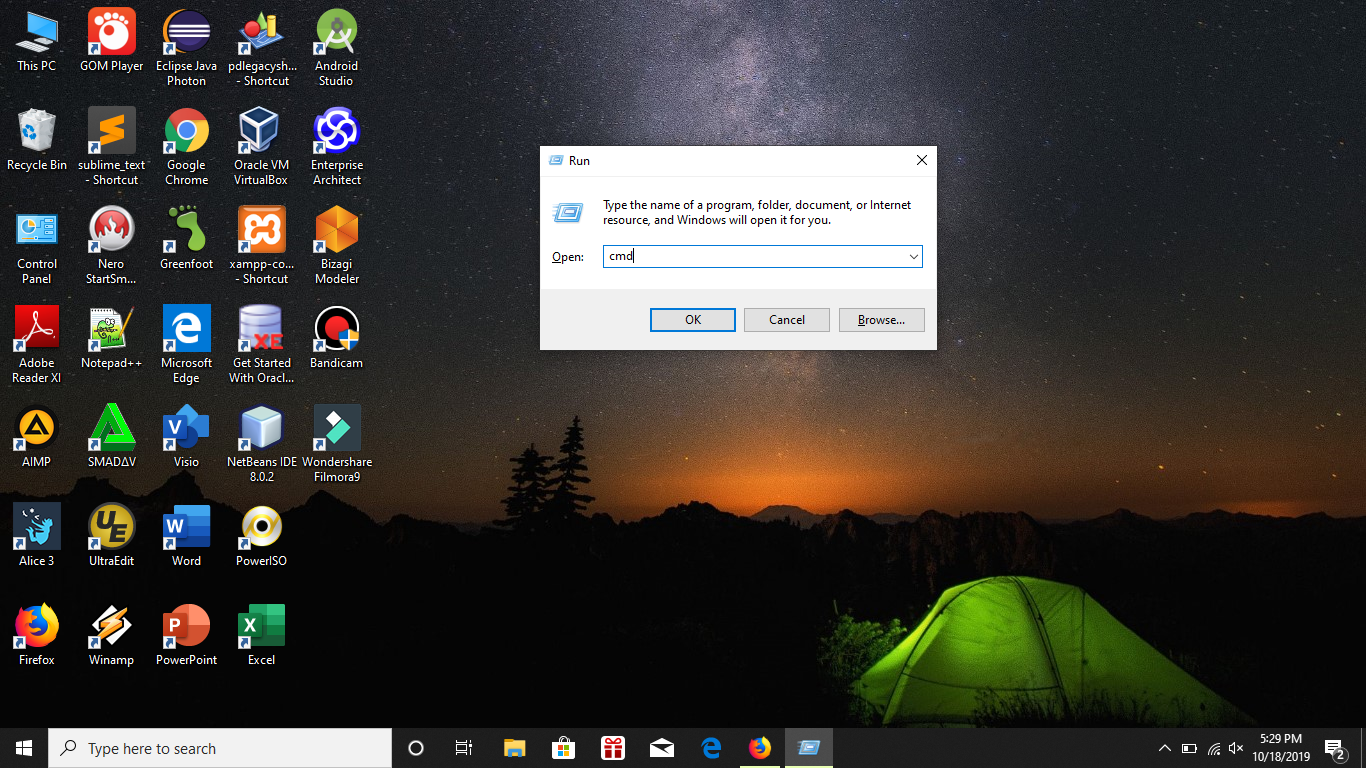
\includegraphics[width=8cm]{image/cmd.png}}
        \end{figure}
    \item Kemudian kita ketikkan Python
        \begin{figure}[h]
            \centerline{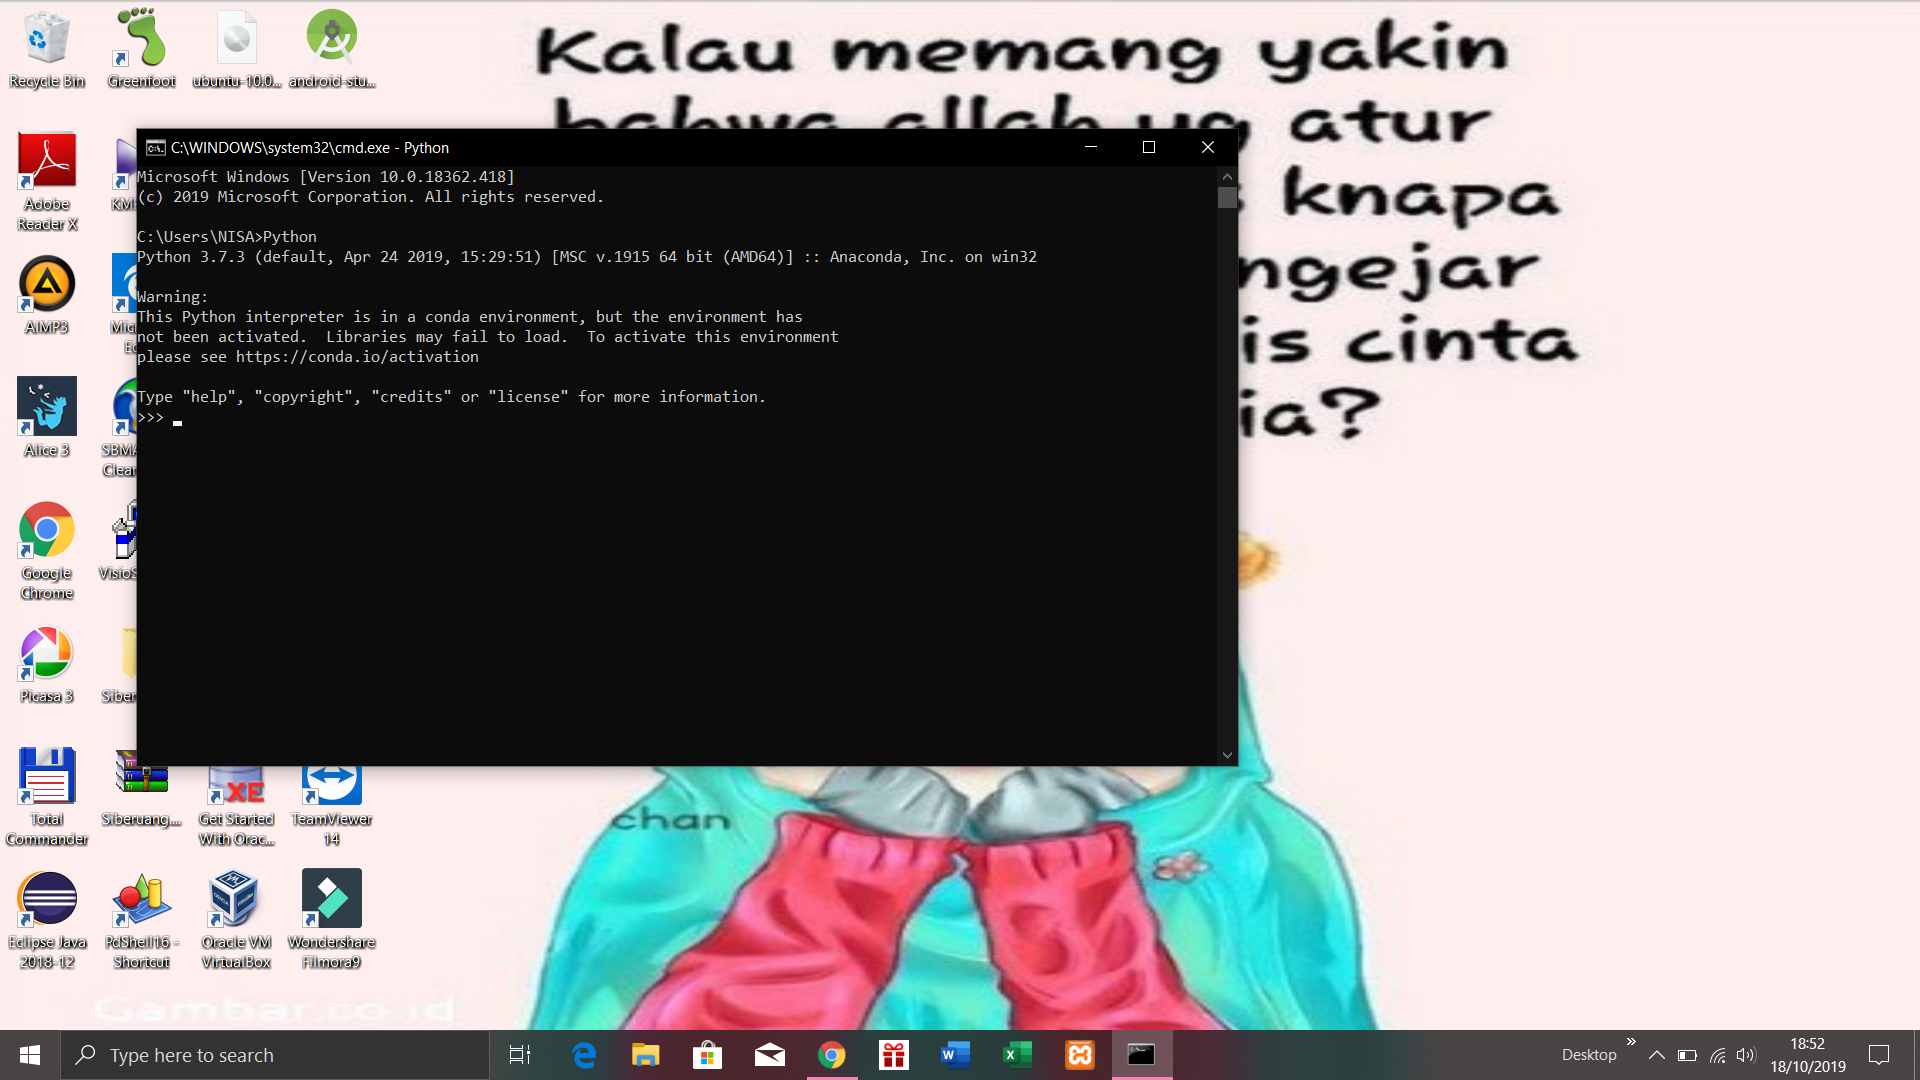
\includegraphics[width=8cm]{image/python.png}}
        \end{figure}
    \newpage \item kemudian kita ketikkan print("Hello World!")
    \paragraph{}
            \centerline{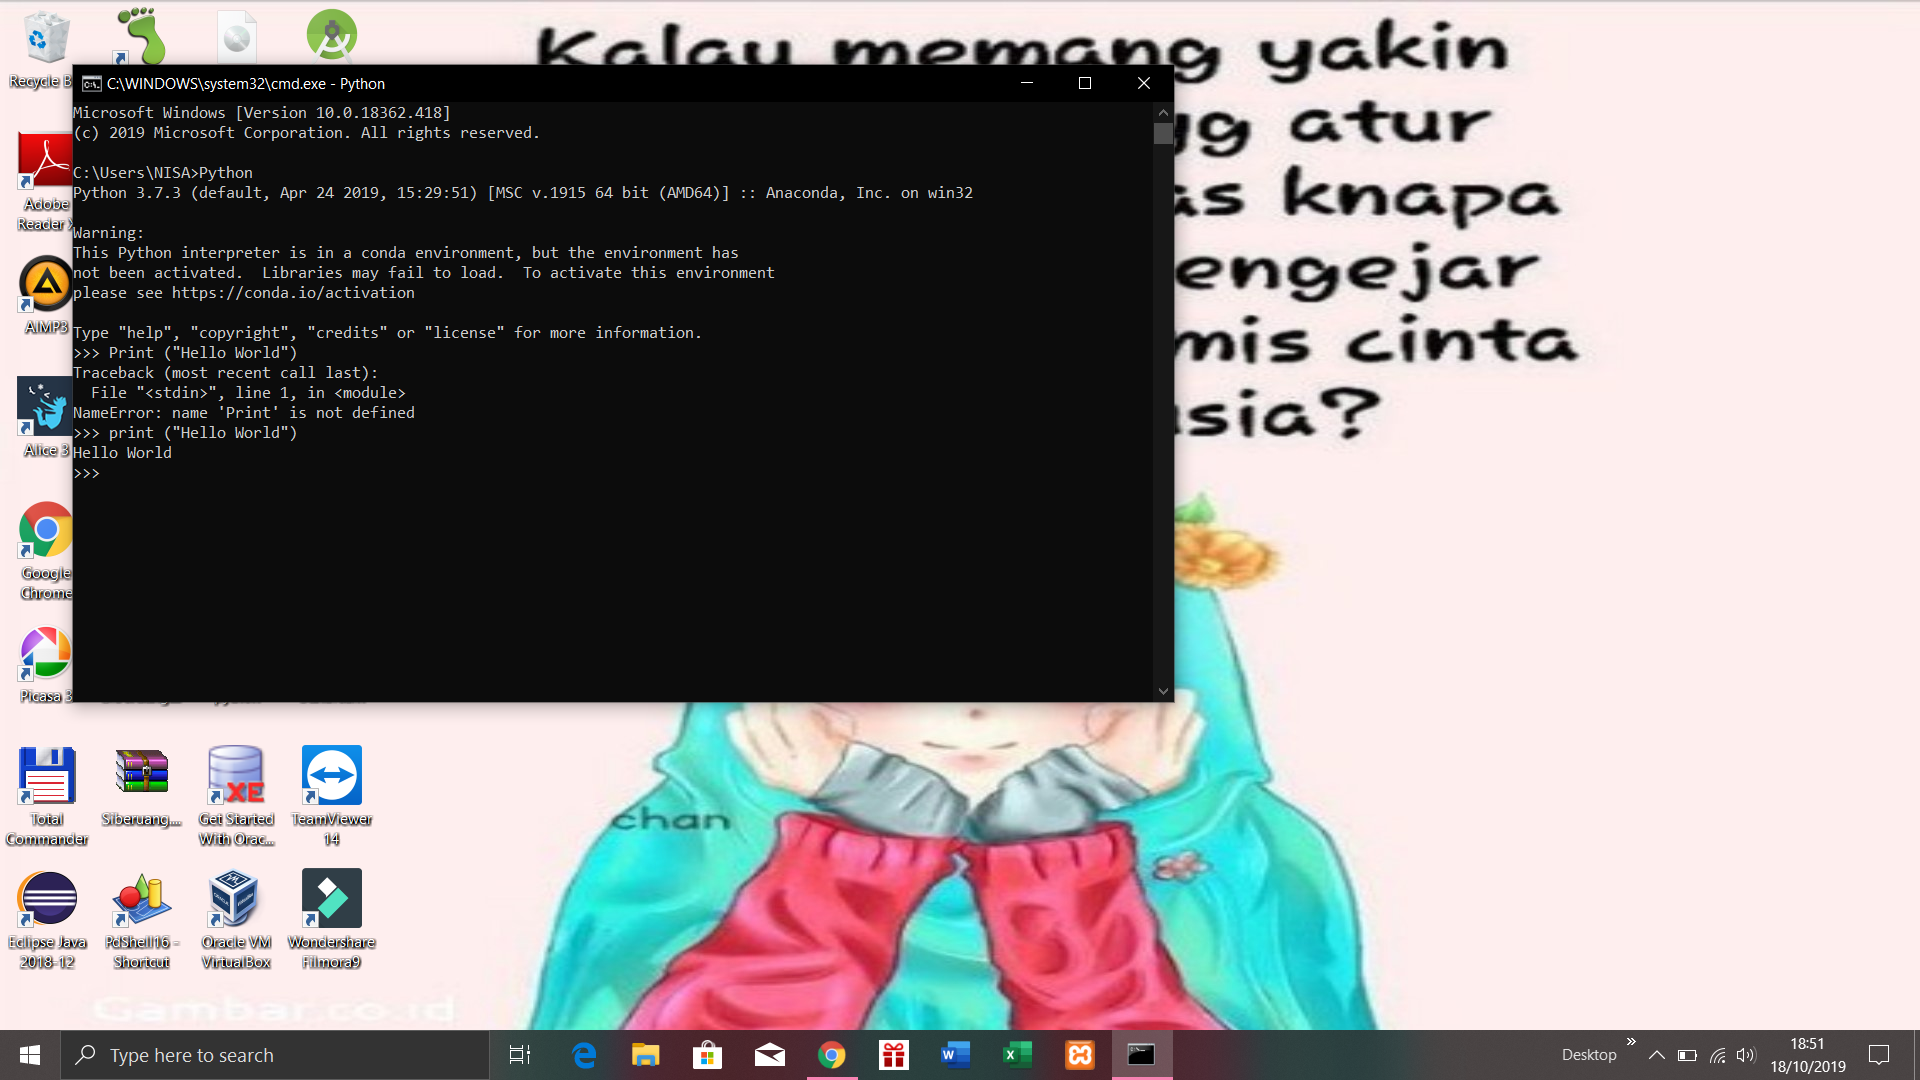
\includegraphics[width=8cm]{image/printhelloworld.png}}
\end{enumerate}
\subsection{Menjalankan dan Mengupdate Anaconda dan Spyder}
\begin{enumerate}
    \item Pertama kita download terlebih dahulu aplikasi Anaconda
    \item Lalu install
    \item Setelah terinstall buka Anaconda
    \item Di dalamnya terdapat Spyder dan lain lain.
    \item Untuk mengupdate Anaconda, silahkan pergi ke cmd lalu ketikkan Conda install -c anaconda python
        \begin{figure}[h]
            \centerline{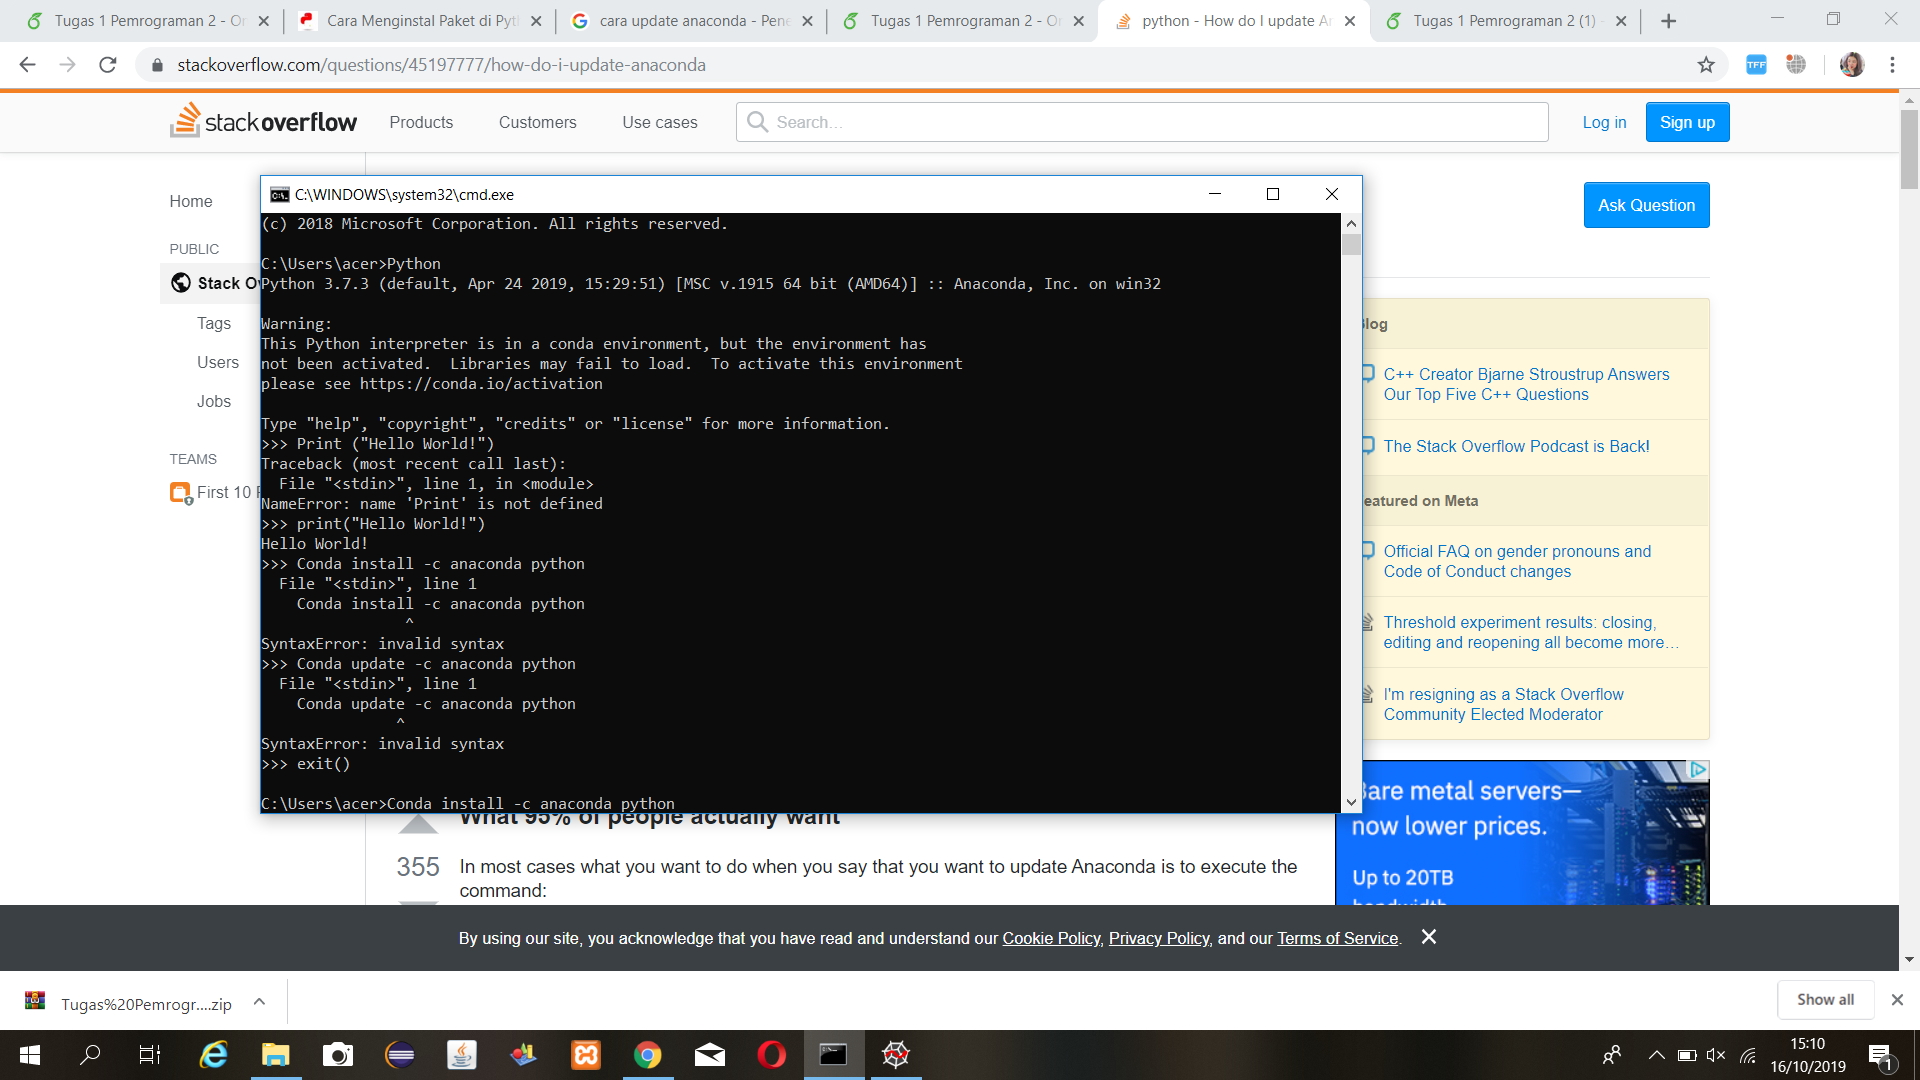
\includegraphics[width=8cm]{image/anacondaupdt.png}}
        \end{figure}
\end{enumerate}
\subsection{Menjalankan Script "Hello World!" di Spyder}
\begin{enumerate}
    \newpage \item Pertama-tama kita buka aplikasi Spyder
    \paragraph{}
            \centerline{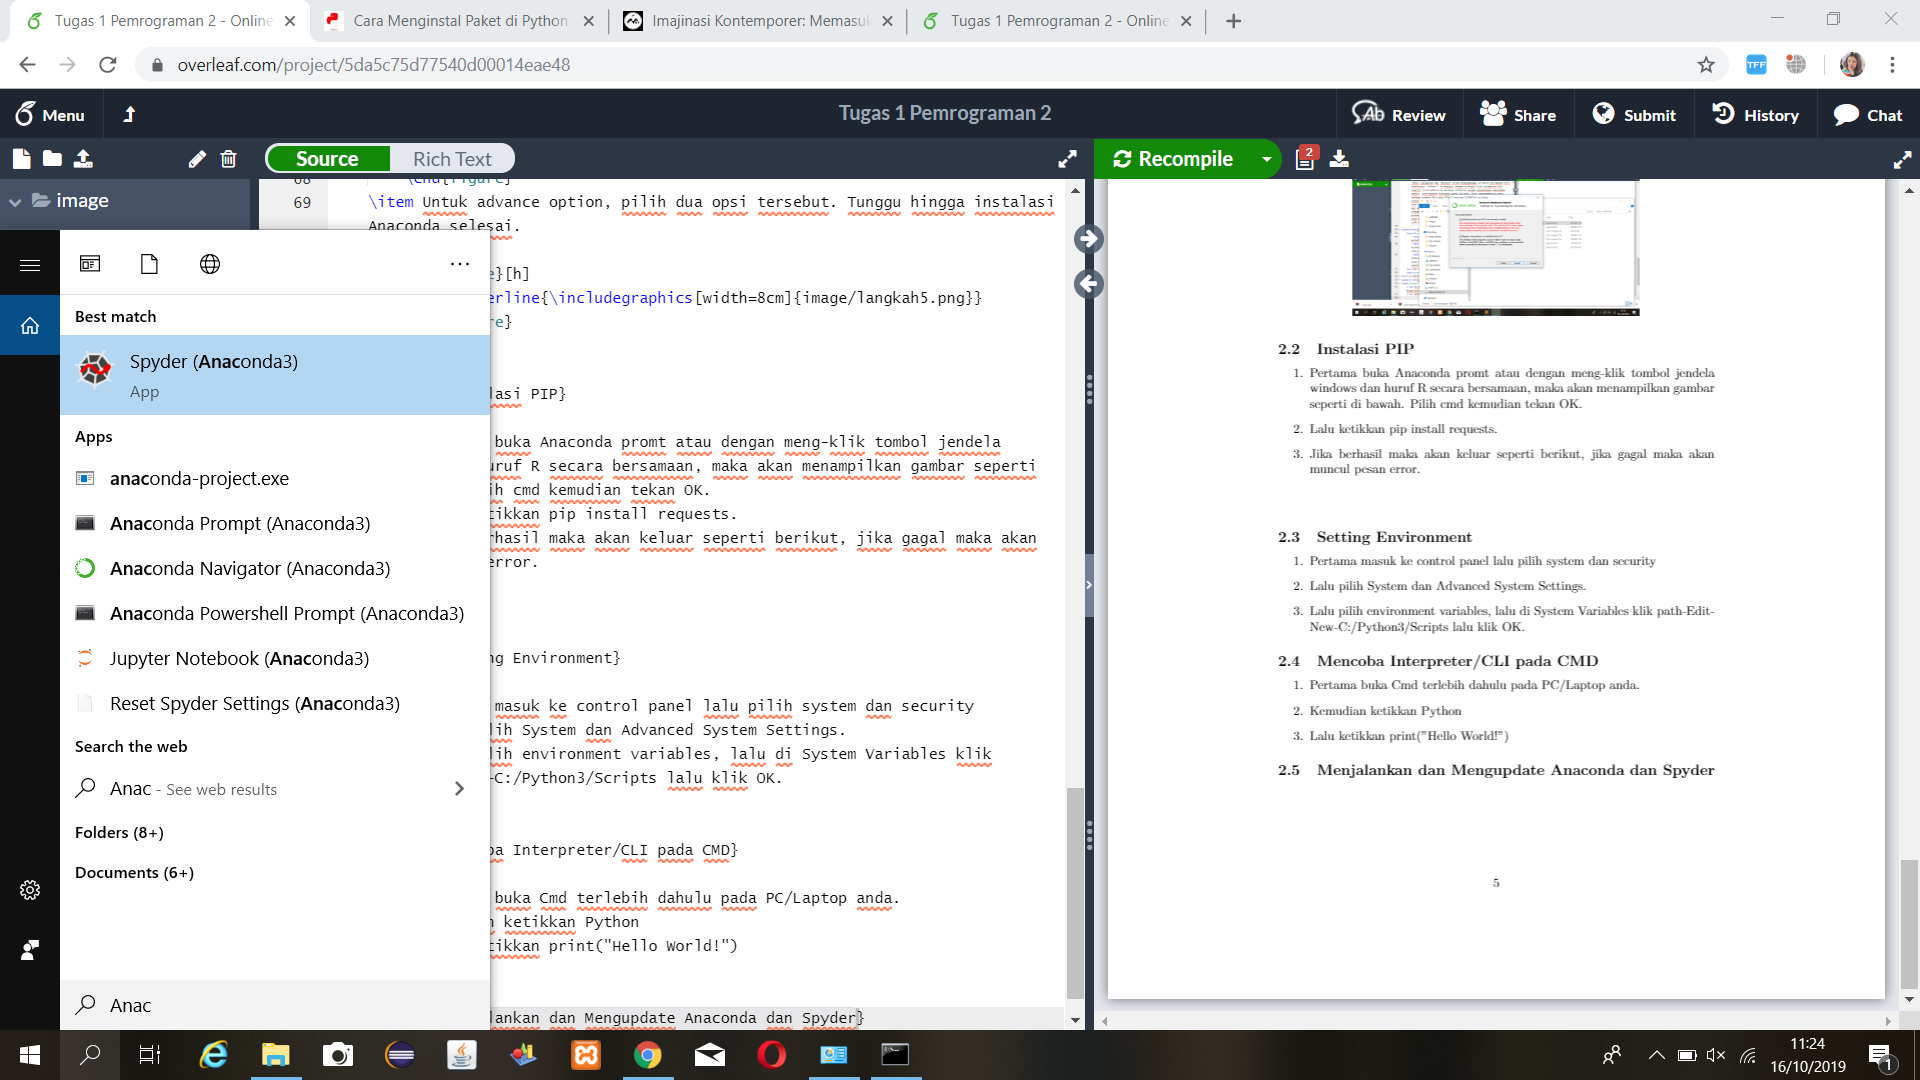
\includegraphics[width=8cm]{image/spyder.png}}
    \item kita ketikkan script seperti berikut
        \begin{figure}[h]
            \centerline{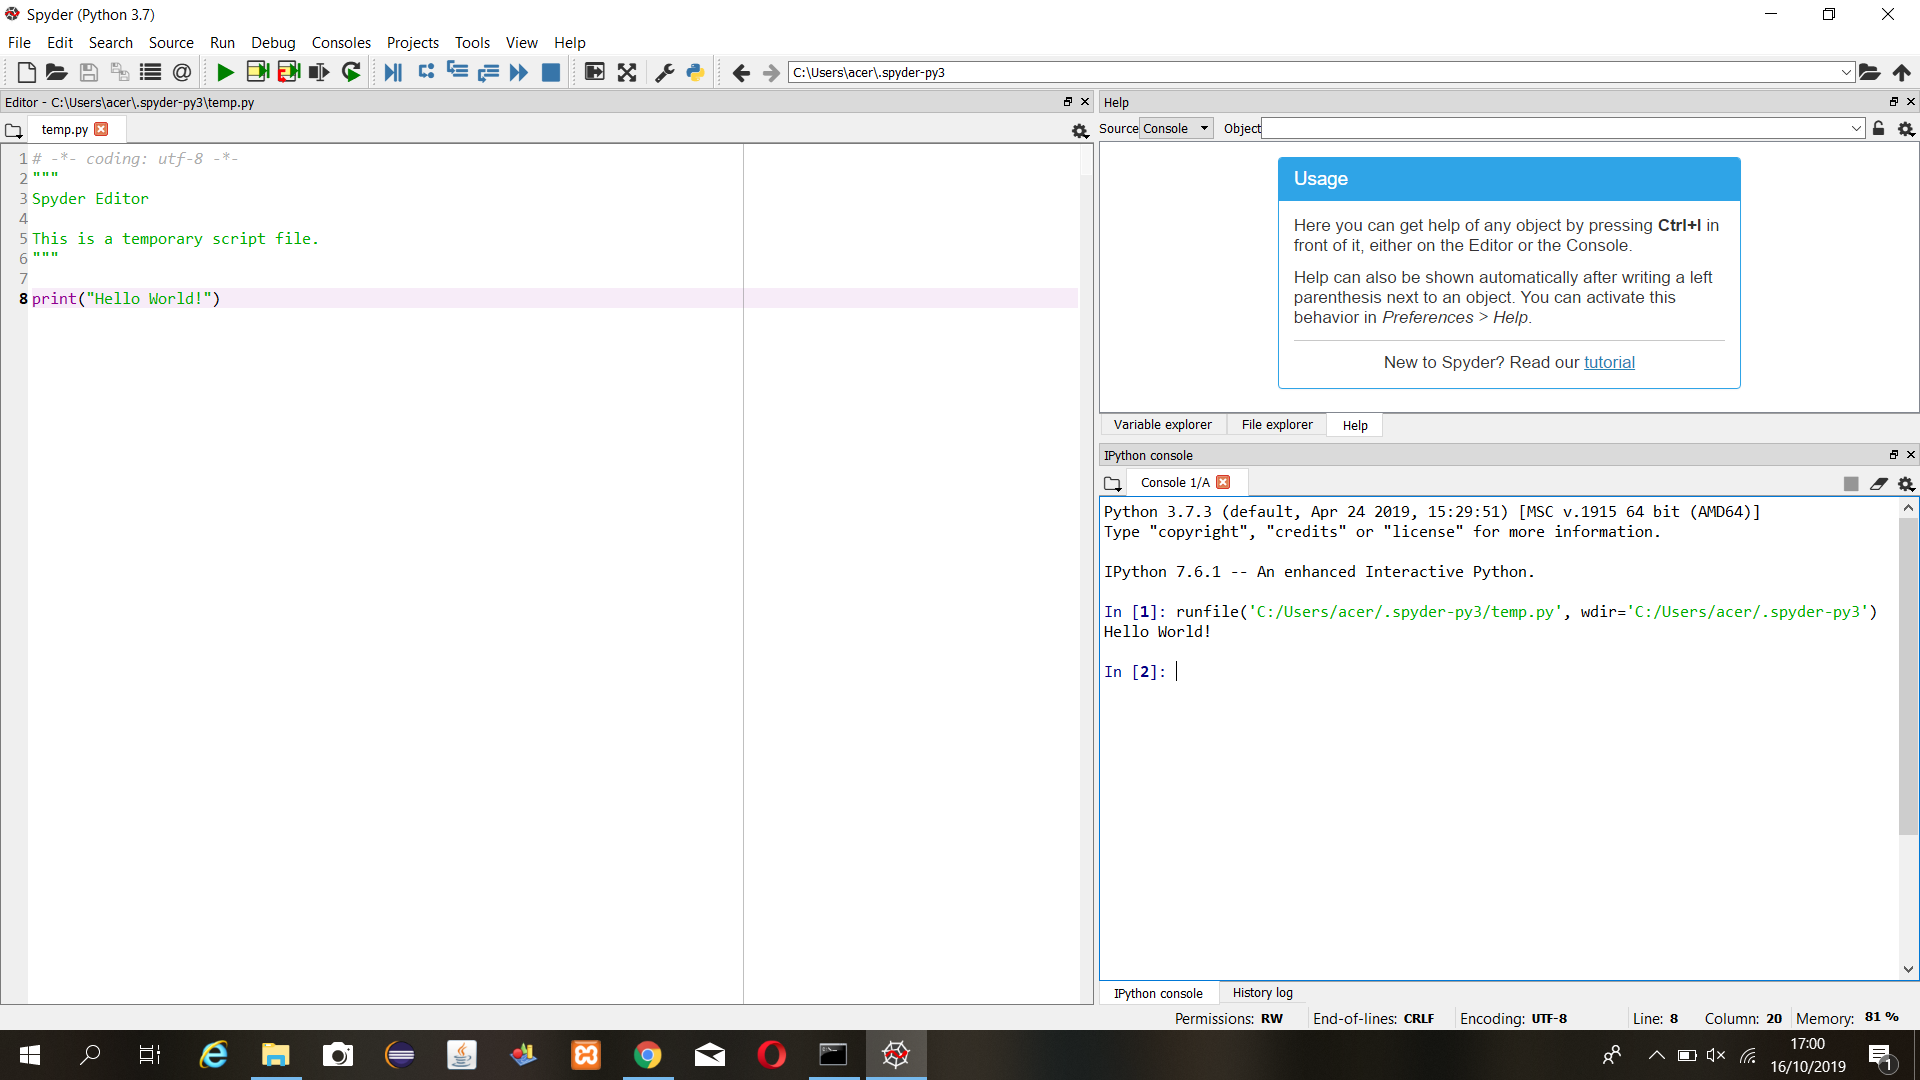
\includegraphics[width=8cm]{image/helloworld.png}}
        \end{figure}
    \item Lalu akan ditampilkan pada console, maka hasilnya "Hello World!"
\end{enumerate}

\subsection{Menjalankan Login Otomatis dengan Library Selenium dan Inputan User}
\begin{enumerate}
    \item Pertama buka cmd terlebih dahulu
    \newpage \item Kemudian kita install Selenium dengan cara ketikkan "pip install selenium"
        \paragraph{}
            \centerline{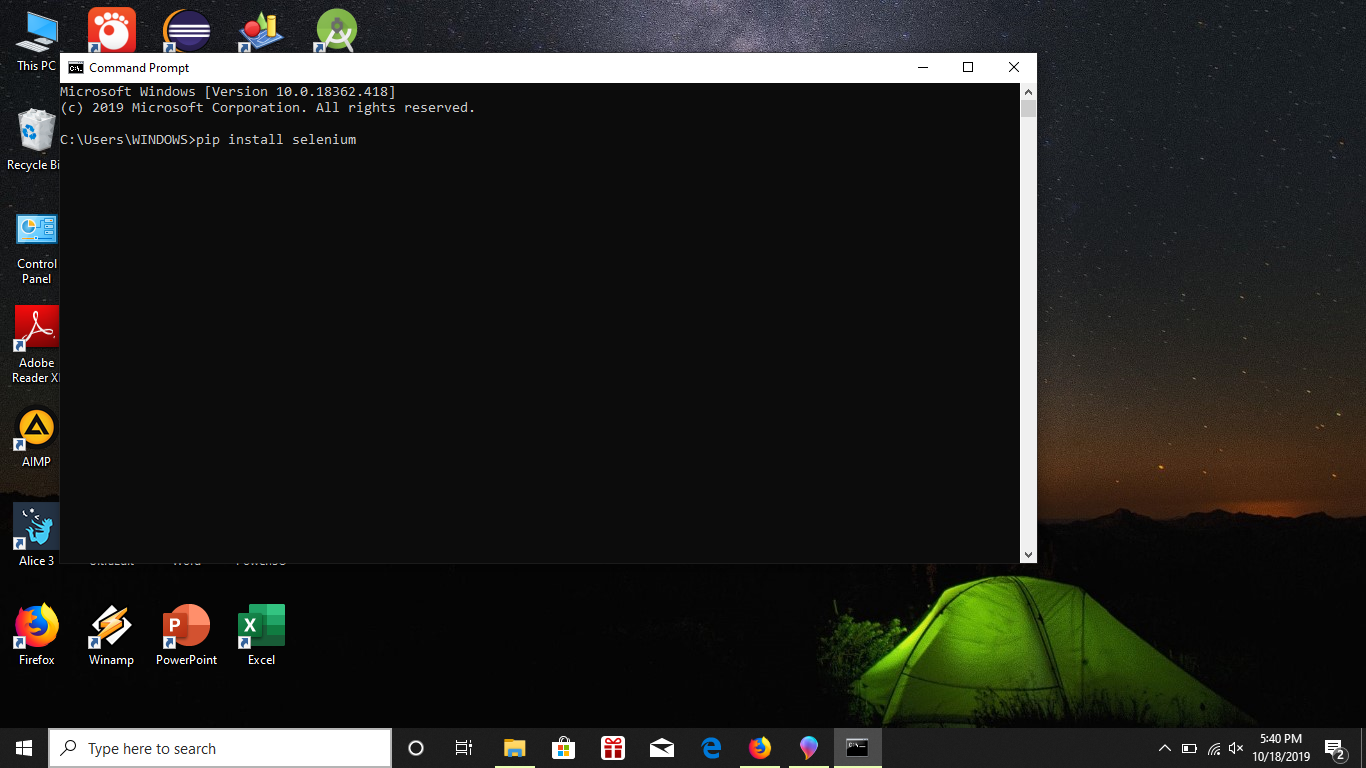
\includegraphics[width=8cm]{image/pipinstallsel.png}}
    \item Lalu kita Download driver, disini saya menggunakan chrome driver. Download driver sesuai browser anda
        \begin{figure}[h]
            \centerline{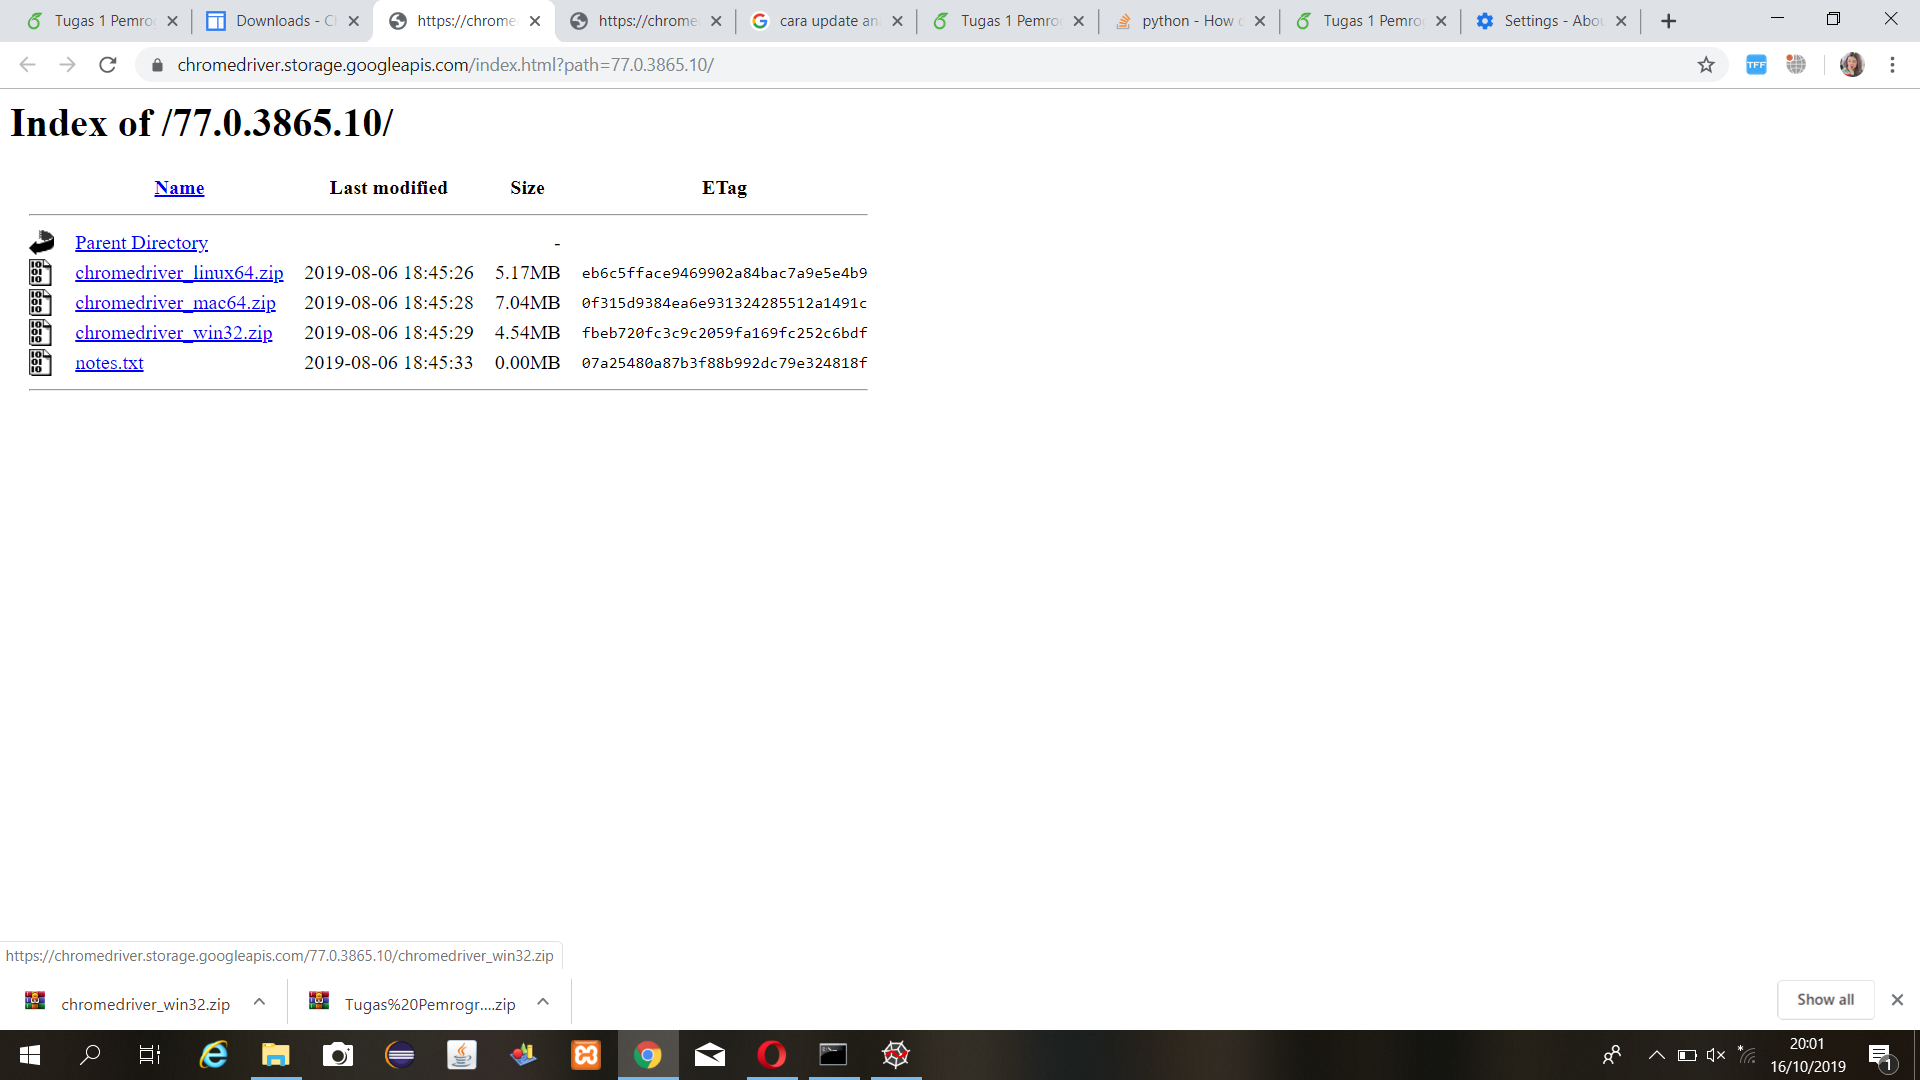
\includegraphics[width=8cm]{image/chromedriver.png}}
        \end{figure}
    \item Selanjutnya kita ketikkan script berikut di Spyder
        \begin{figure}[h]
            \centerline{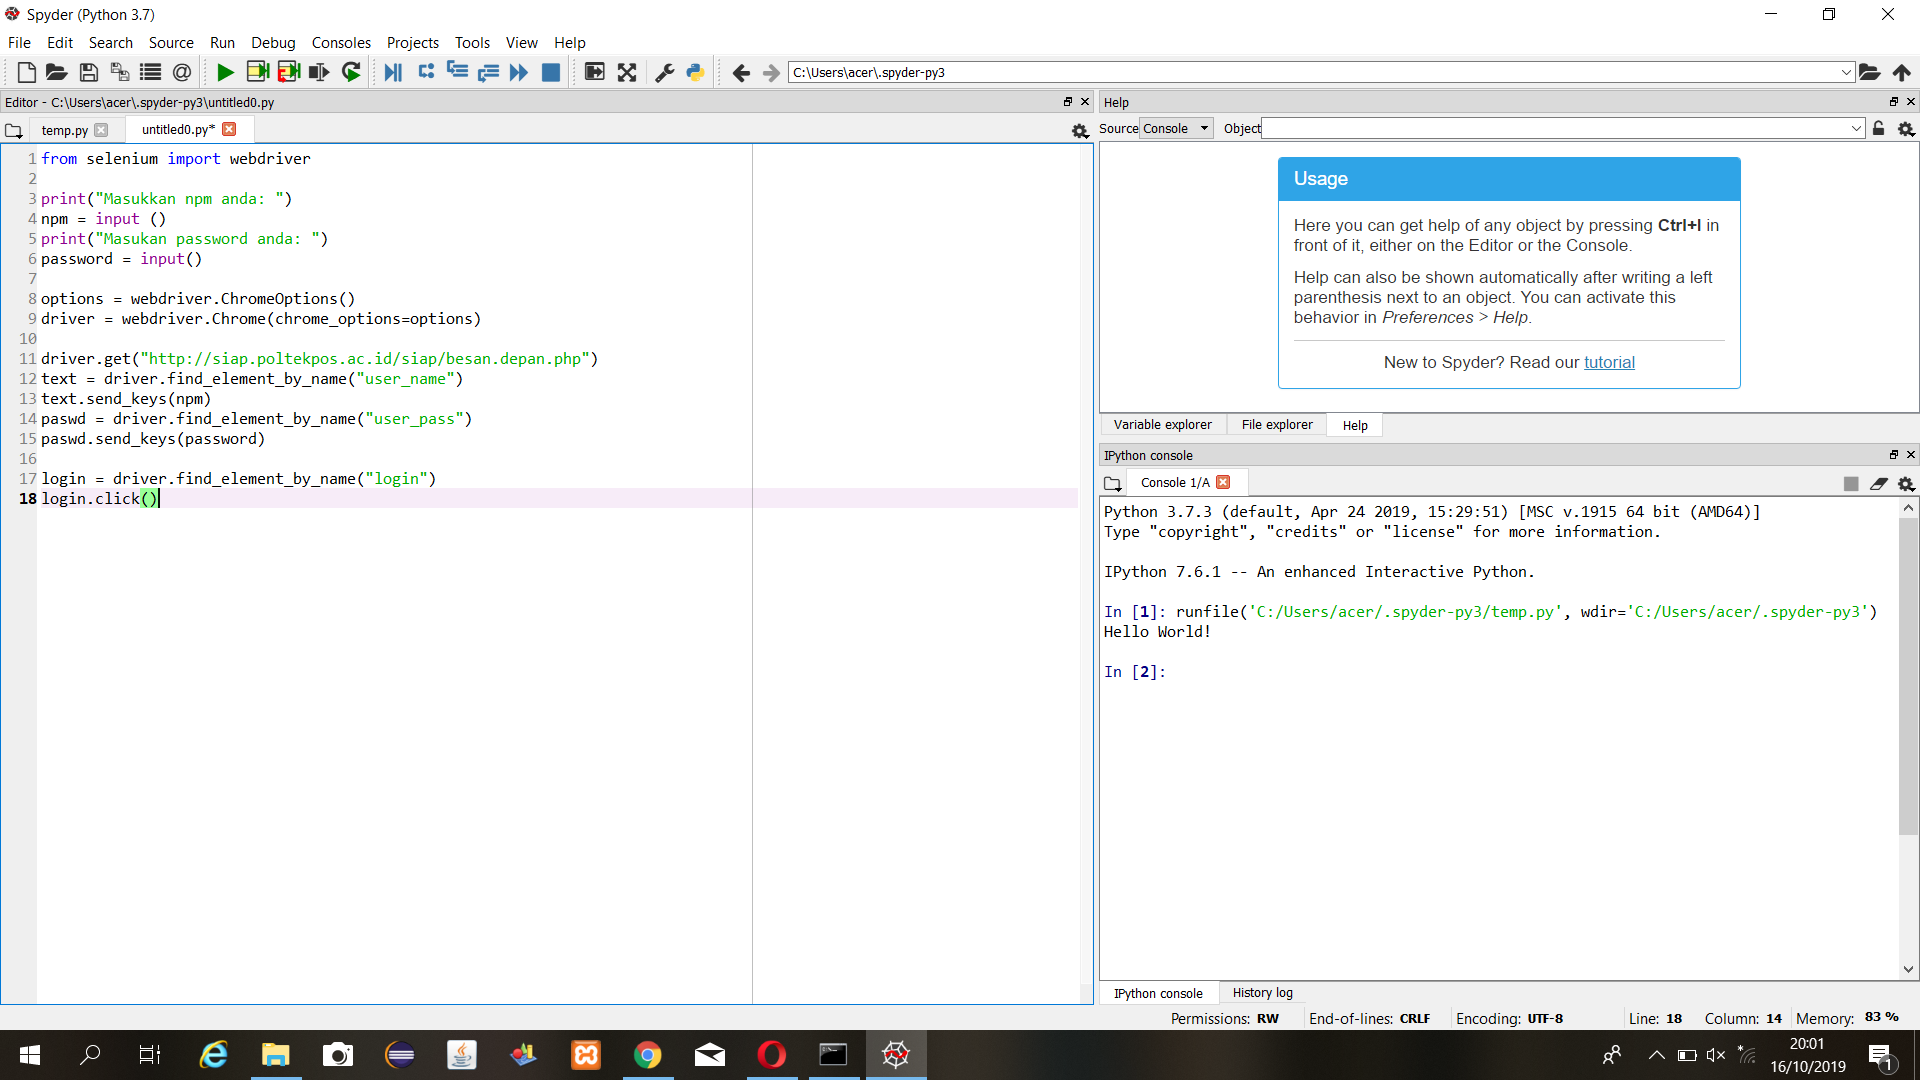
\includegraphics[width=8cm]{image/scriptsele.png}}
        \end{figure}
    \item Kemudian kita run kan, setelah itu akan login otomatis ke browser yang akan kita tujui
\end{enumerate}

\subsection{Cara Menggunakan Variabel Explorer pada Spyder}
\begin{enumerate}
    \item Buka aplikasi Spyder pada PC/laptop anda
    \item Pada program tersebut, tambahkan variabel a yang bertipe integer nilai nya bebas, begitu pula dengan variabel b
    \item Variabel c tersebut merupakan hasil dari penjumlahan variabel a dan b, c = a+b
    \item Hasilnya akan diperlihatkan dengan jelas pada variabel explore
        \begin{figure}[h]
            \centerline{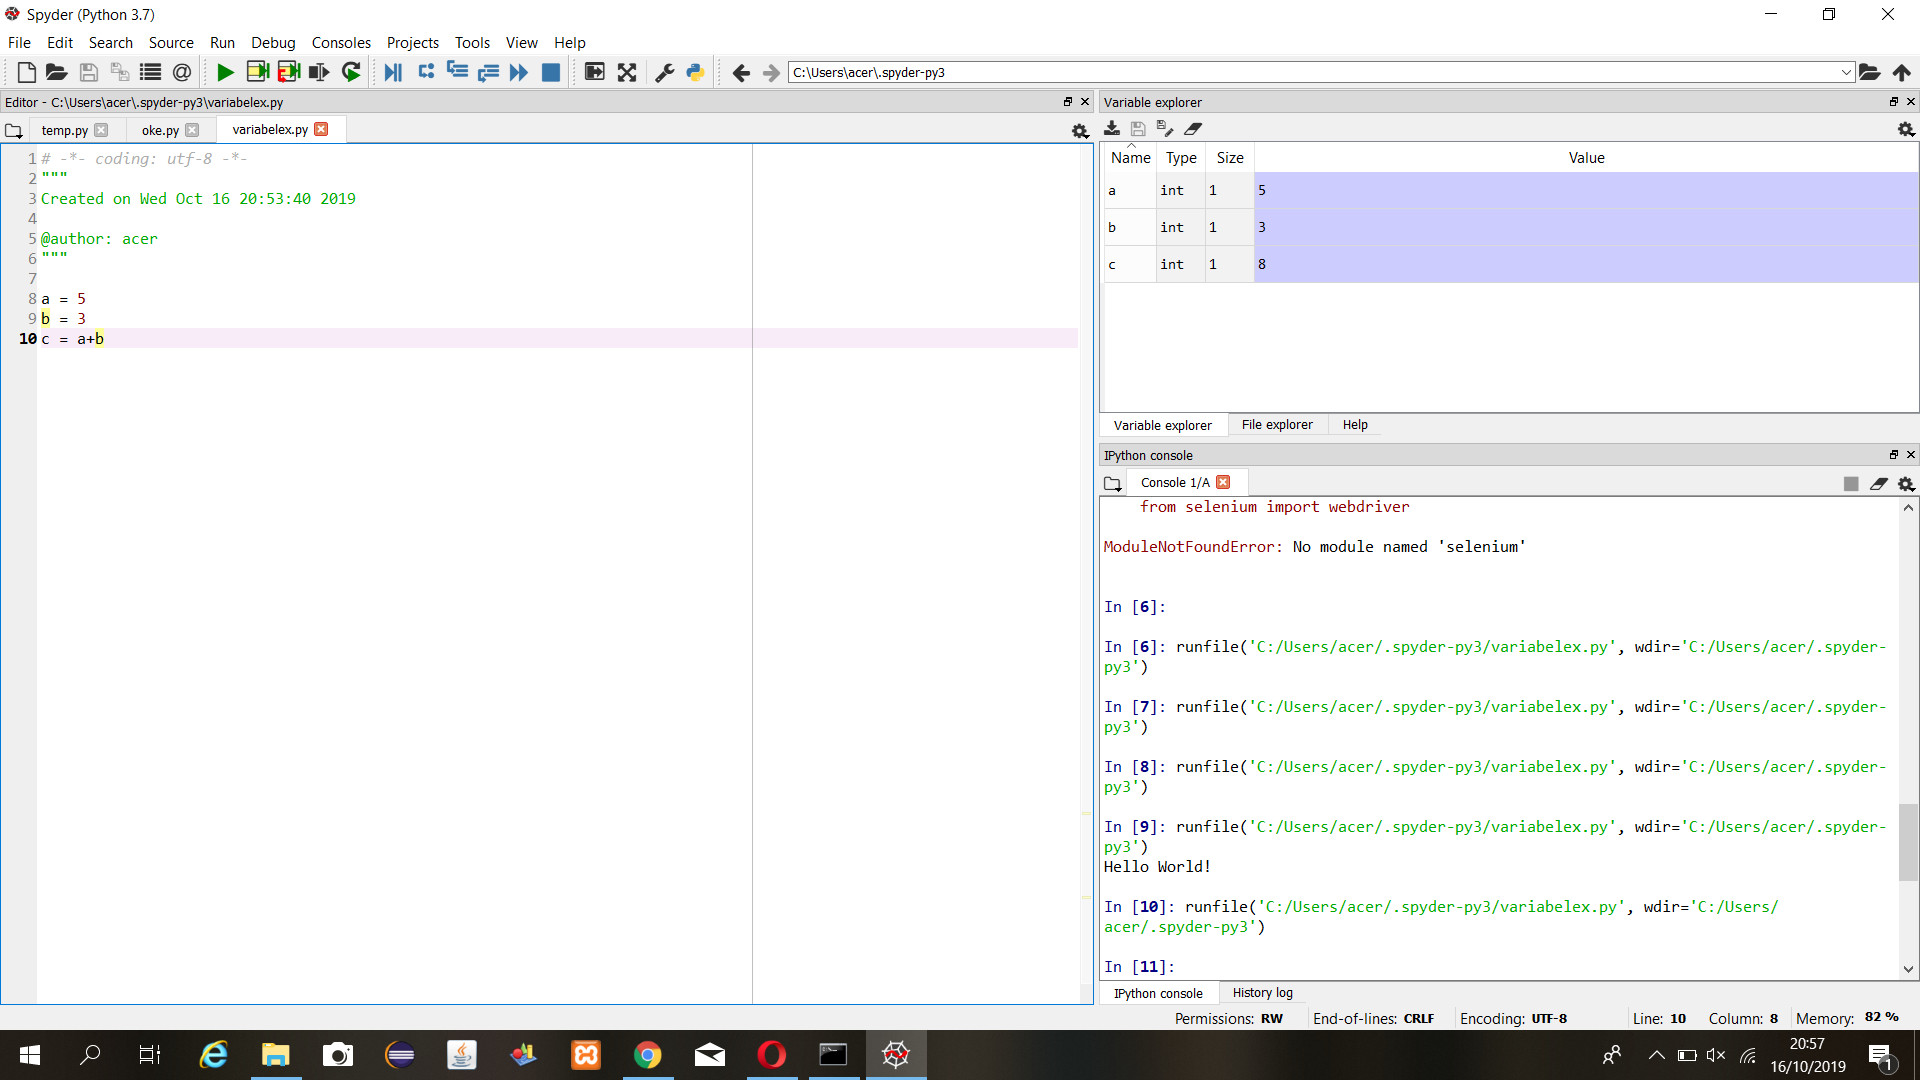
\includegraphics[width=8cm]{image/variabelex.png}}
        \end{figure}
\end{enumerate}

\section{Identasi}
\subsection{Pengertian Identasi}
\paragraph{}
    Identasi merupakan bagian awal dari sebuah paragraf yang menjorok ke dalam pada setiap baris paragraf.
\subsection{Jenis-Jenis Error Identasi yang Dapat Ditemukan}
\begin{enumerate}
    \item Identasi If
    \item Identasi Else
    \item Identasi Elif
\end{enumerate}
\subsection{Contoh Eror dan Benar}
\begin{enumerate}
    \newpage \item Contoh Error
    \paragraph{}
        \centerline{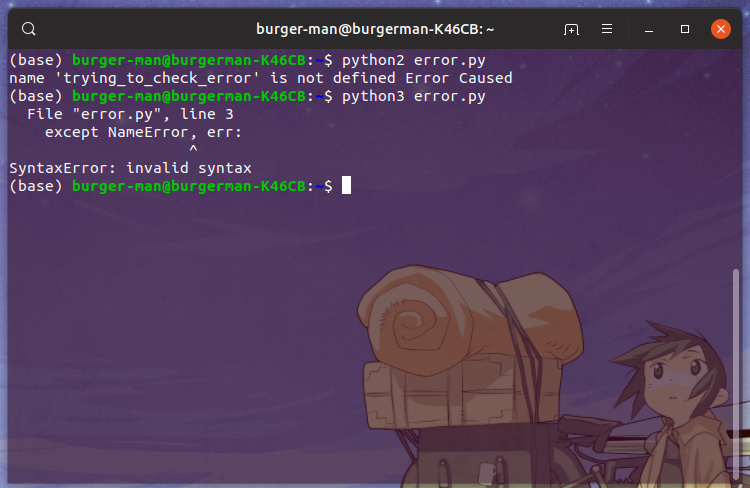
\includegraphics[width=8cm]{image/error.png}}
    \item Contoh Benar
    \begin{figure}[h]
            \centerline{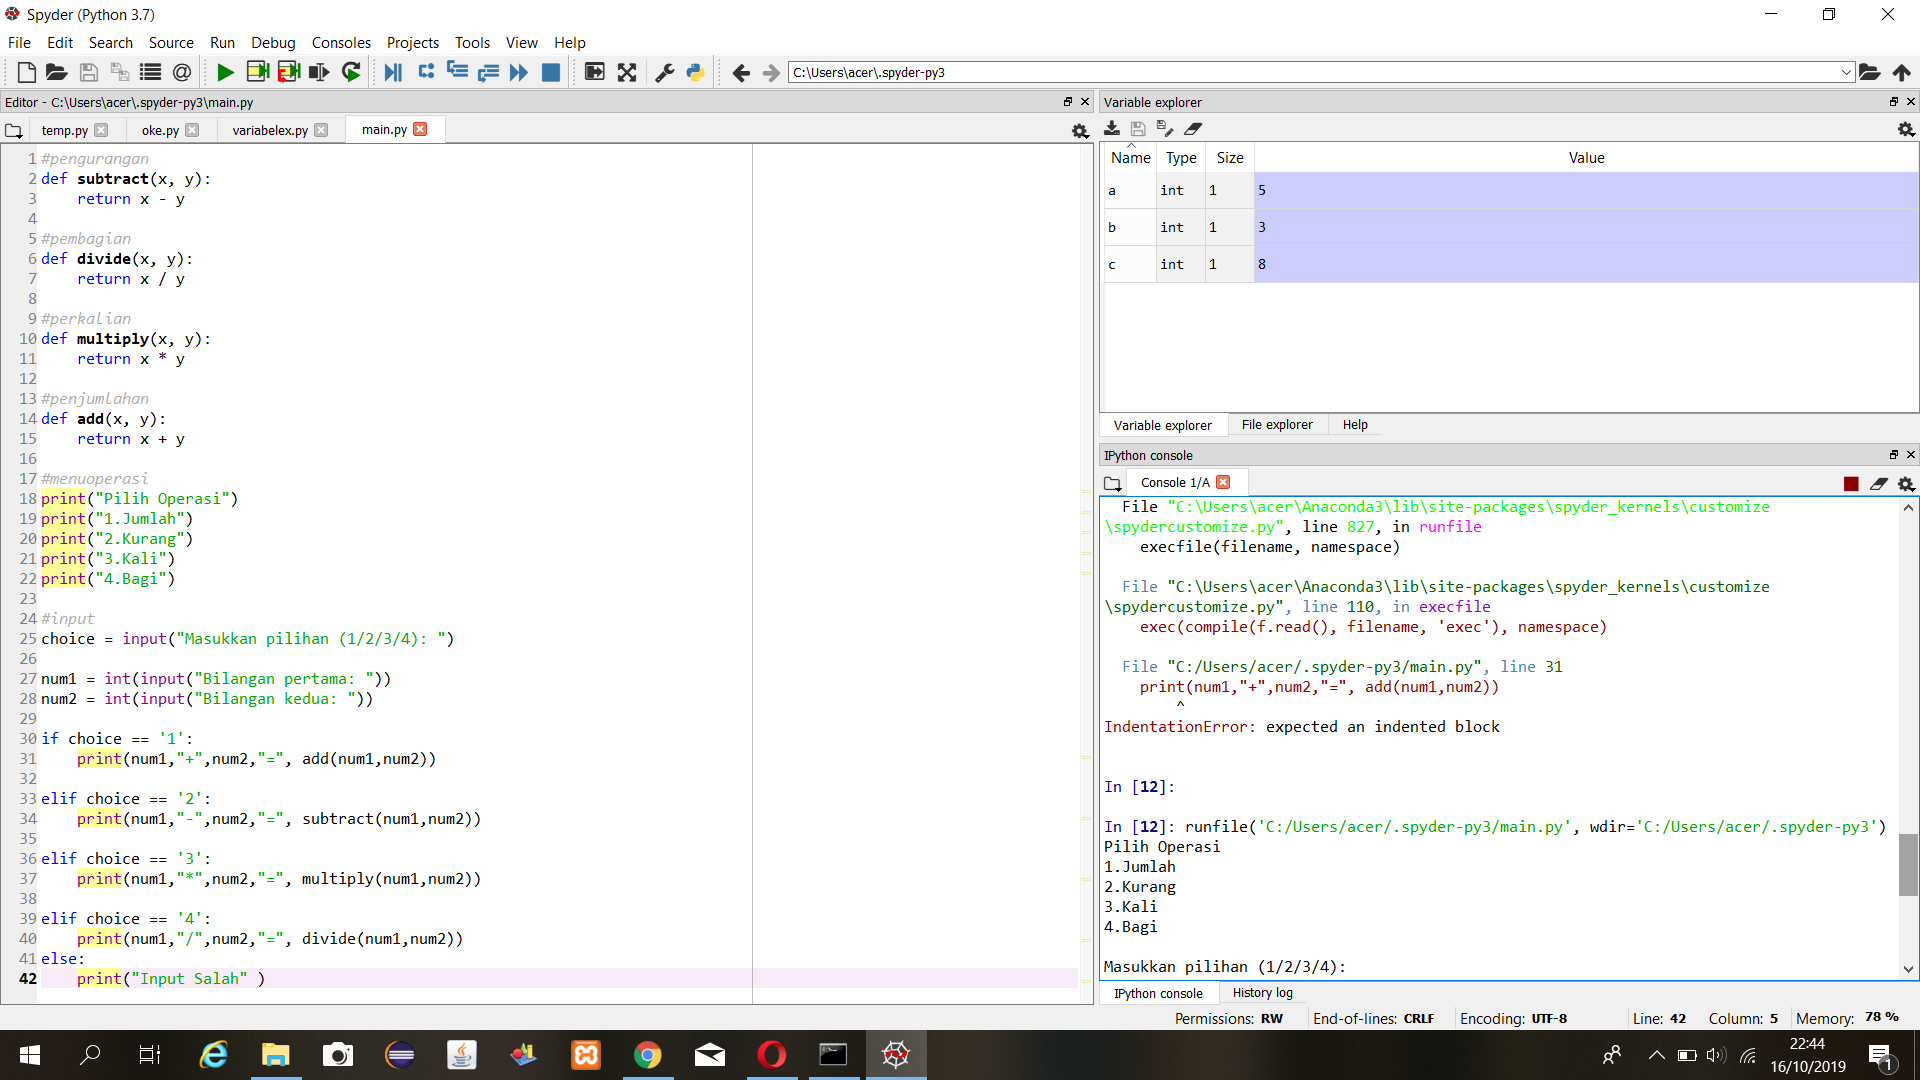
\includegraphics[width=8cm]{image/contohbenar.png}}
        \end{figure}
\end{enumerate}
\section{Link Youtube channel "https://youtu.be/pNWStMLQZNQ" }
\end{document}
